\chapter{فرانت‌اند}
    \section{ساختار راهنمای وب‌سایت}
    این راهنما به شما کمک می‌کند تا با تمام بخش‌های وب‌سایت آشنا شوید و بتوانید از قابلیت‌های آن به‌طور کامل استفاده کنید. وب‌سایت Polaris با هدف ارائه‌ی یک بستر کاربرپسند و تعاملی طراحی شده است که کاربران را قادر می‌سازد تا اطلاعات شبکه را مشاهده کرده، گزارش‌ها را بررسی کنند و به ابزارهای مدیریتی پیشرفته دسترسی داشته باشند.  
    راهنما به‌گونه‌ای ساختار یافته که شما از اولین ورود به صفحه‌ی اصلی تا استفاده از امکانات پیشرفته، مسیر مشخصی را دنبال کنید. در هر بخش، توضیحات همراه با مراحل عملی ارائه شده‌اند تا تجربه‌ی استفاده شما روان و بدون ابهام باشد.  
    \section{شروع به کار}
    \begin{itemize}
    	\item  معرفی کوتاهی از وب‌سایت و عملکردهای کلیدی آن: وب‌سایت Polaris یک پلتفرم تحت وب برای مدیریت، مانیتورینگ و تحلیل داده‌های شبکه است. این سامانه با رابط کاربری ساده و مدرن، امکاناتی همچون مشاهده‌ی نقشه‌ی پوشش، بررسی وضعیت لحظه‌ای شبکه، دسترسی به گزارش‌های دقیق و استفاده از ابزارهای مدیریتی را فراهم می‌کند. هدف اصلی این وب‌سایت، ارائه‌ی اطلاعات دقیق و به‌روز به کاربران، همراه با تجربه‌ی کاربری سریع و کارآمد است. این وب‌سایت در آدرس \url{http://45.149.77.43:5174/} قرار گرفته است.
    	\item  صفحه فرود: توضیح بخش‌های اصلی صفحه فرود.
    \end{itemize}
    \section{مدیریت حساب کاربری}
    \begin{itemize}
    	\item \textbf{ثبت‌نام:} برای ایجاد حساب کاربری در نسخه تحت‌وب \lr{Polaris}، در صفحه اصلی وب‌سایت روی دکمه \lr{Login} کلیک کنید:
	    	\begin{center}
	    		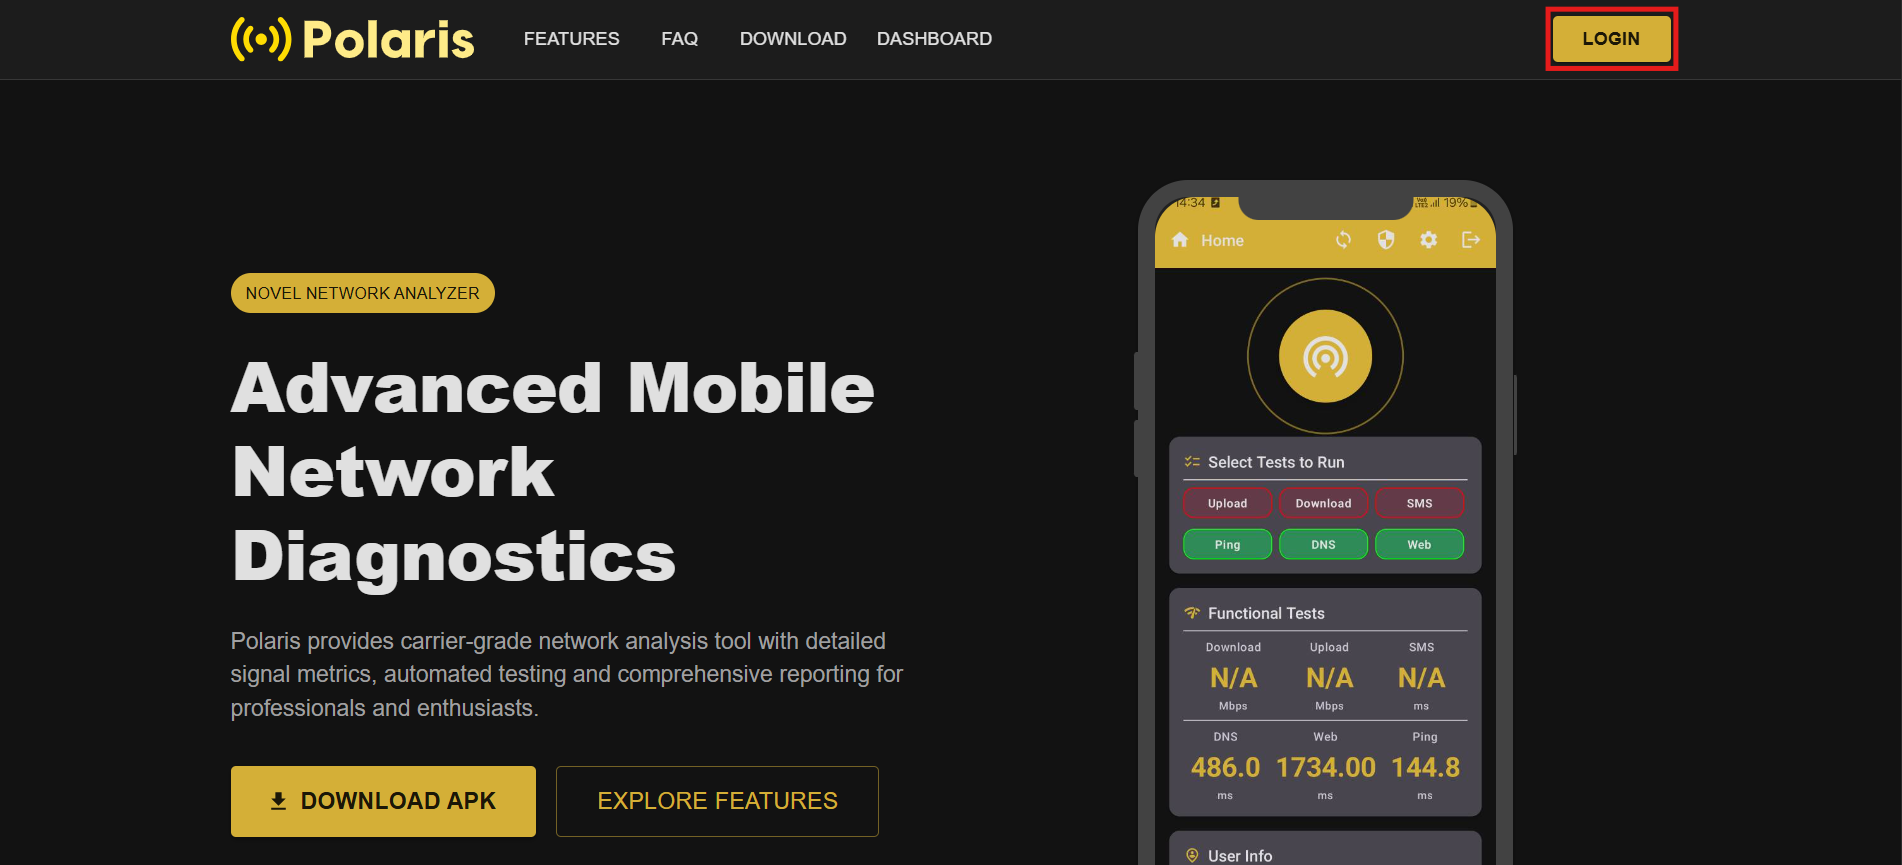
\includegraphics[width=\textwidth]{images/fr-landing.png}
	    	\end{center}
    	سپس به صفحه زیر منتقل می‌شوید که در این صفحه نیز نیاز است بر روی لینک \lr{Sign Up} کلیک کنید:
    		\begin{center}
    			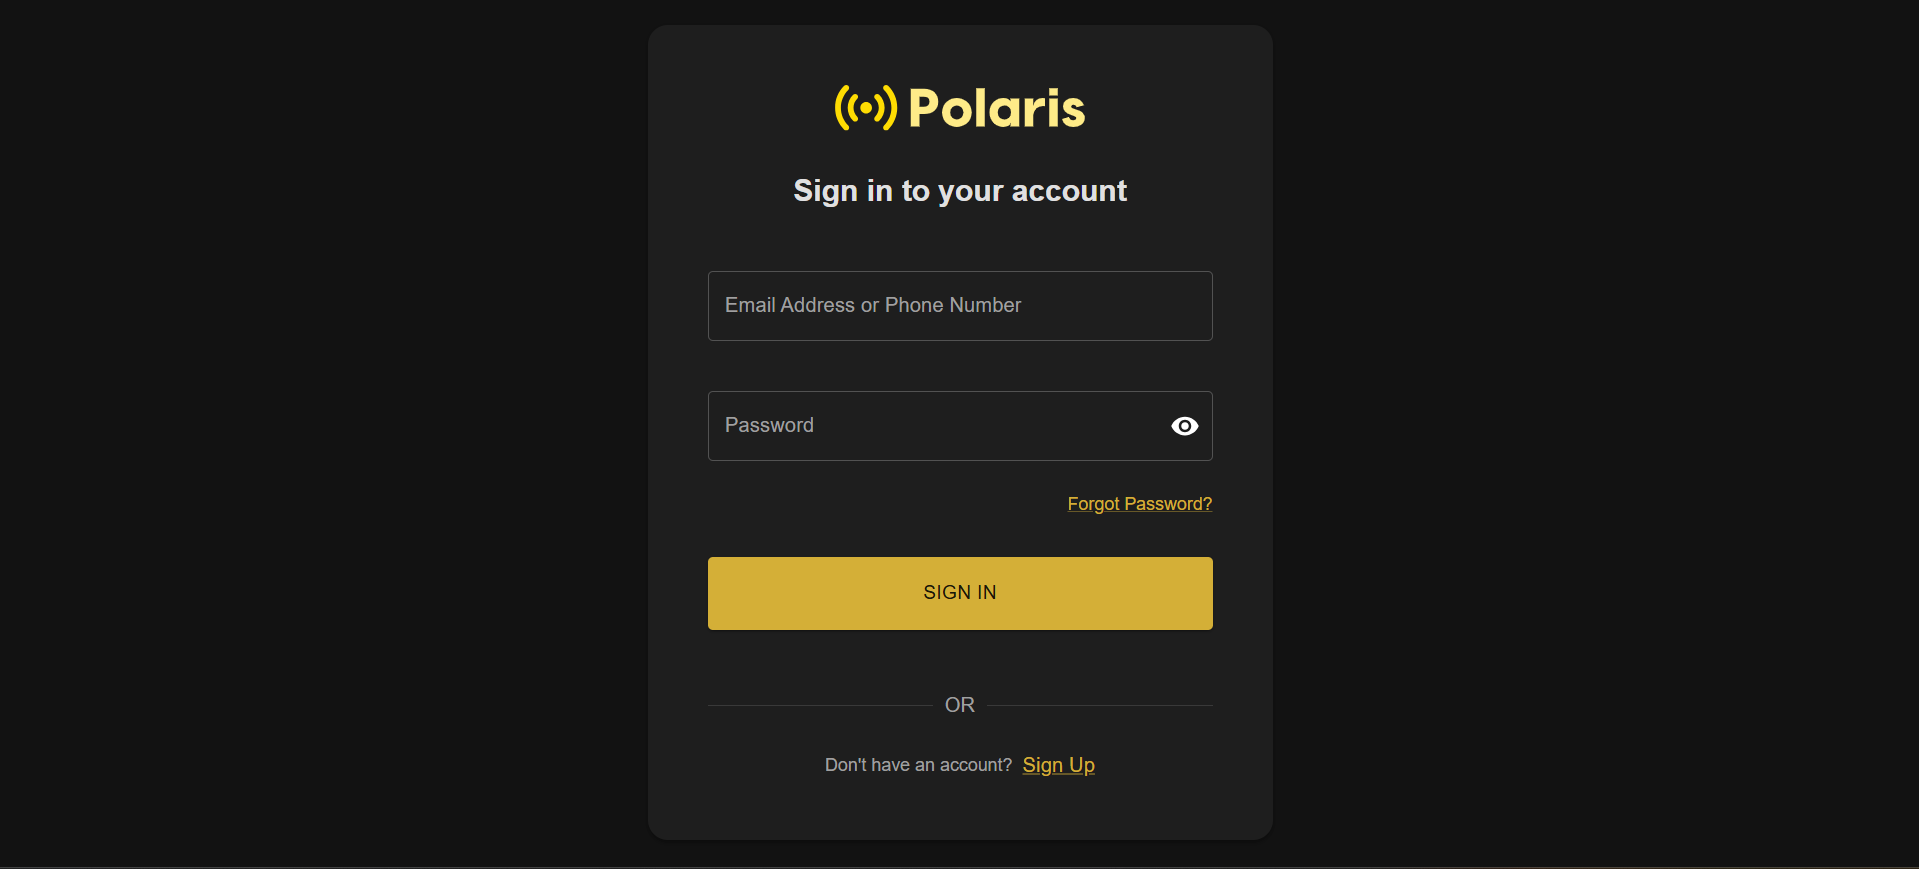
\includegraphics[width=\textwidth]{images/fr-login-empty.png}
    		\end{center} 
    		پس از کلیک بر روی لینک \lr{Sign Up} به صفحه زیر منتقل می‌شوید:
    		\begin{center}
    			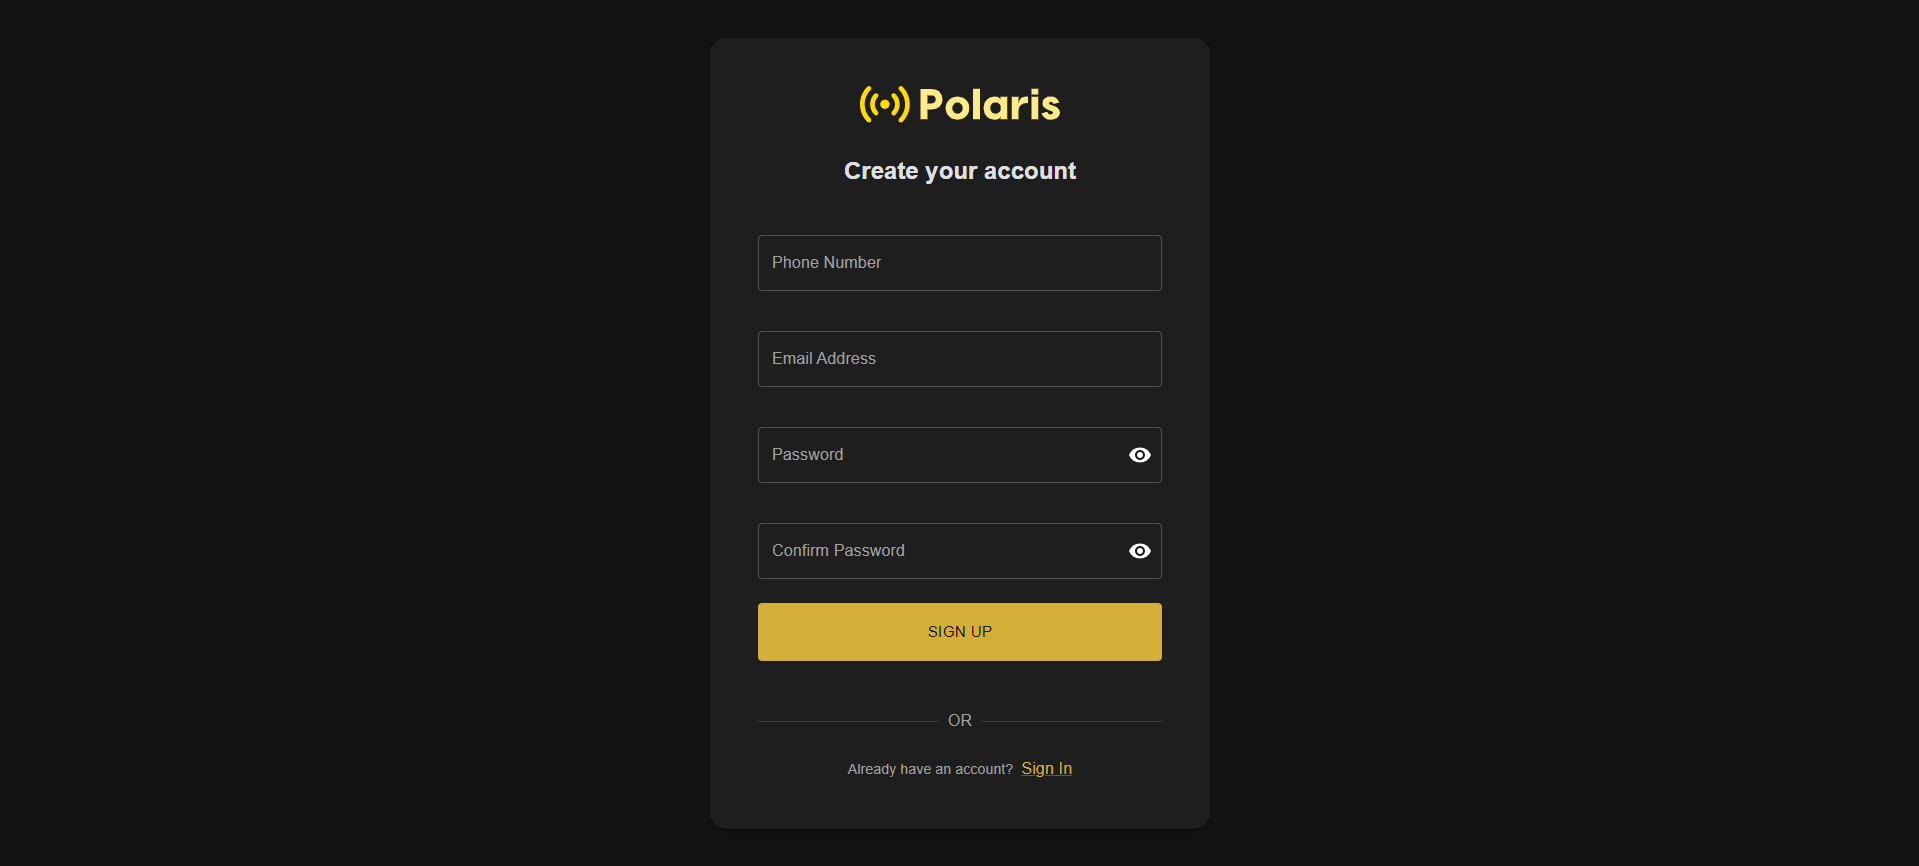
\includegraphics[width=\textwidth]{images/fr-signup-empty.png}
    		\end{center}
    		در این صفحه در صورت تمایل و داشتن حساب می‌توانید به صفحه Login برگردید.
    	\begin{itemize}
    		\item \textbf{پر کردن فرم ثبت‌نام:}  
    		در این صفحه، اطلاعات خواسته‌شده شامل پست الکترونیک، شماره تلفن همراه و گذرواژه را وارد کنید. شماره همراه باید به فرمت \lr{09xxxxxxxxx} و گذرواژه باید حداقل 8 کاراکتر (شامل حروف و اعداد) باشد. پس از تکمیل فرم، روی دکمه \lr{Sign Up} کلیک کنید. در صورت وجود خطا، پیام مناسب نمایش داده می‌شود و در غیر این صورت، پیام موفقیت آمیز بودن نمایش داده می‌شود:
    			\begin{center}
    				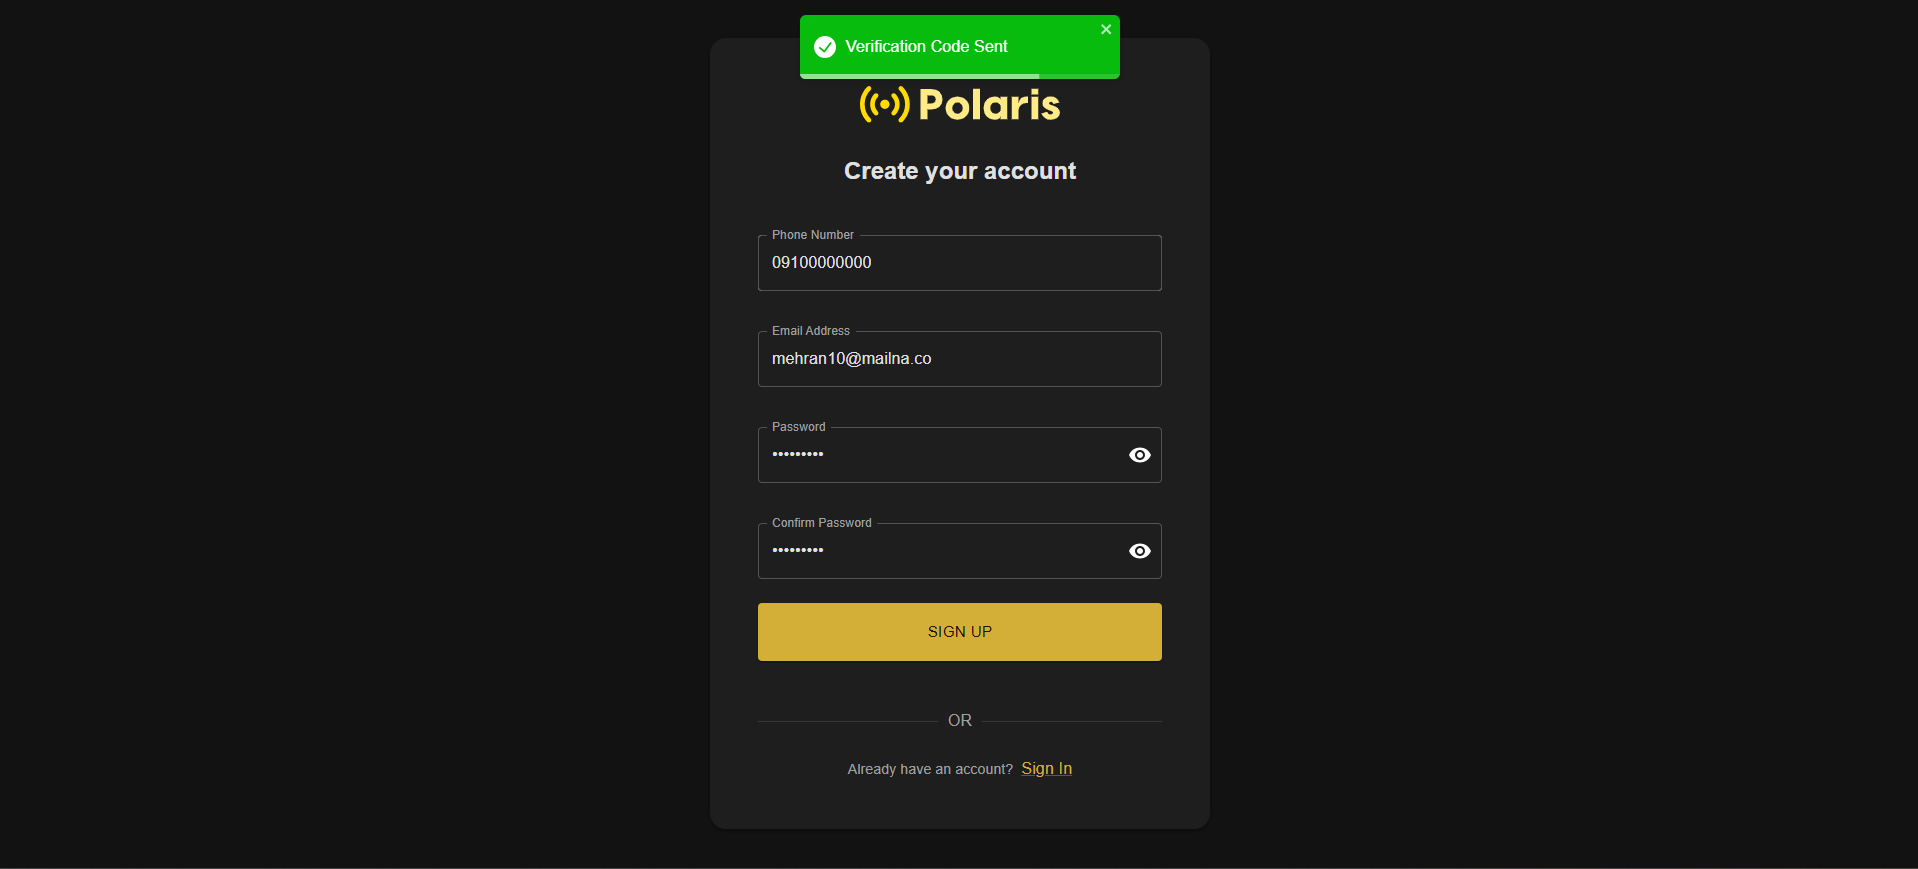
\includegraphics[width=\textwidth]{images/fr-signup-success.png}
    			\end{center}
    		\item \textbf{تأیید آدرس ایمیل:}  
    		پس از ارسال فرم ثبت‌نام، در صورت موفقیت آمیز بودن به صفحه تأیید منتقل می‌شوید:
    		\begin{center}
    			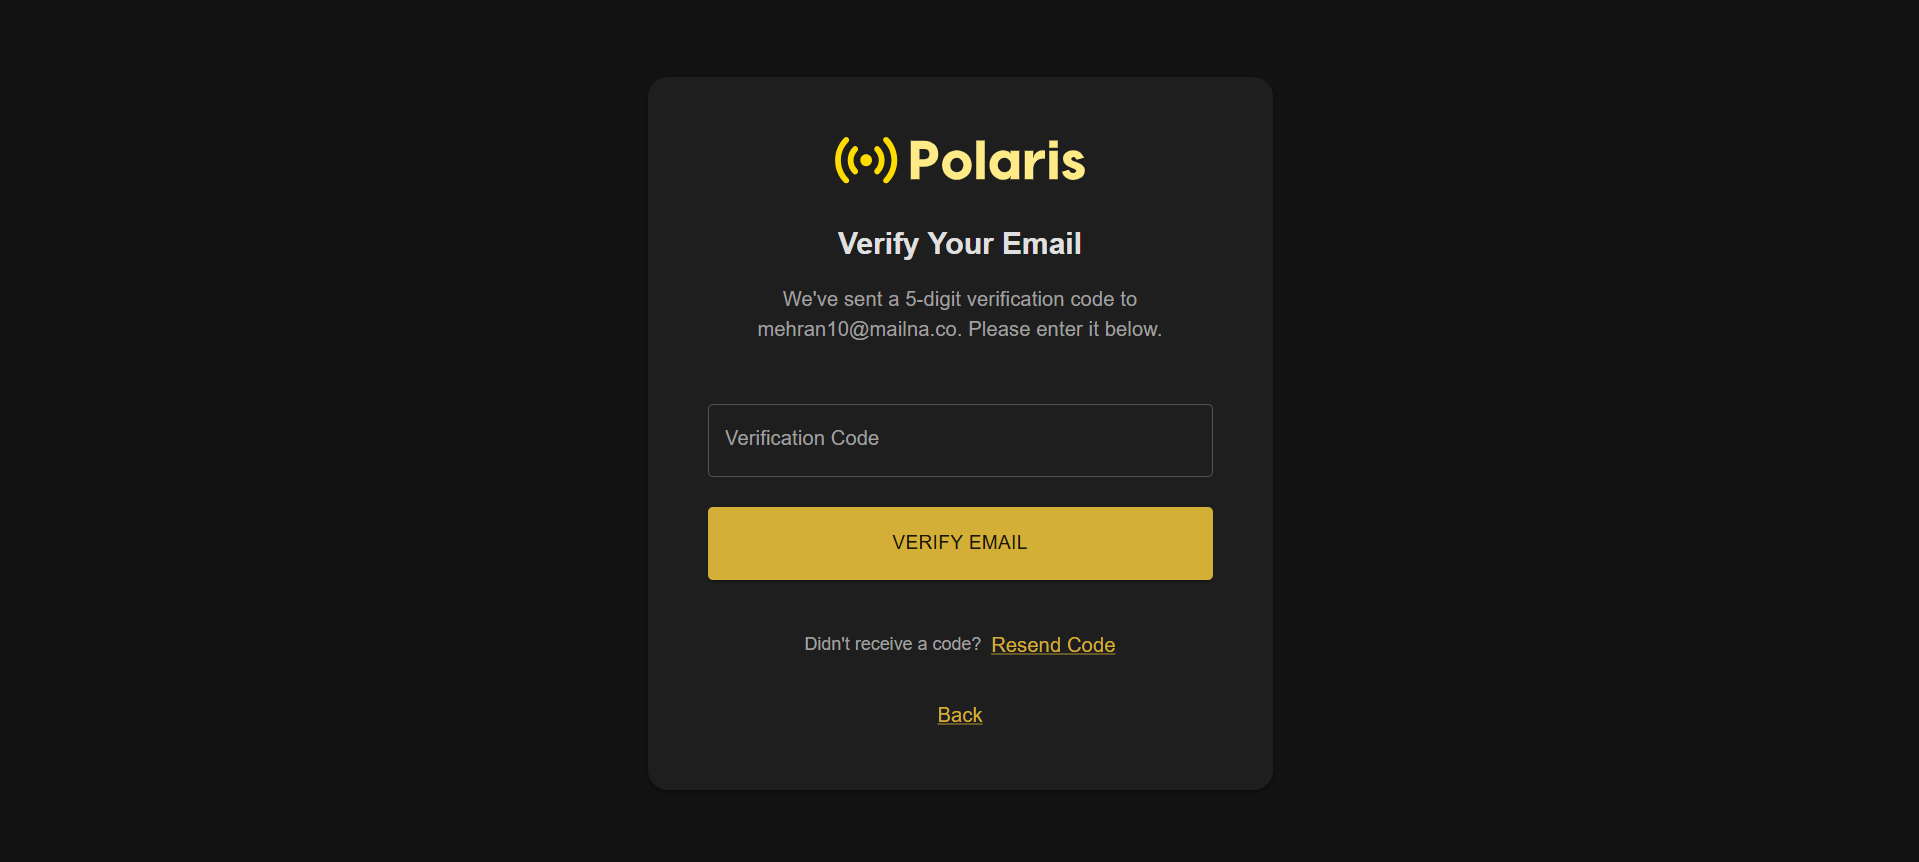
\includegraphics[width=\textwidth]{images/fr-verify-empty.png}
    		\end{center}
    		در این بخش، کد ۵ رقمی ارسال‌شده به ایمیلی که در مرحله قبل وارد کرده‌اید را وارد کنید. در صورت عدم دریافت کد، می‌توانید روی لینک \lr{Resend Code} کلیک کنید. همچنین، امکان بازگشت به صفحه ثبت‌نام با کلیک بر روی \lr{Back} وجود دارد.  
    		پس از وارد کردن کد صحیح، پیام موفقیت‌آمیز بودن ایجاد حساب نمایش داده شده و با یک تأخیر کوتاه به داشبورد منتقل می‌شوید:
    		\begin{center}
    			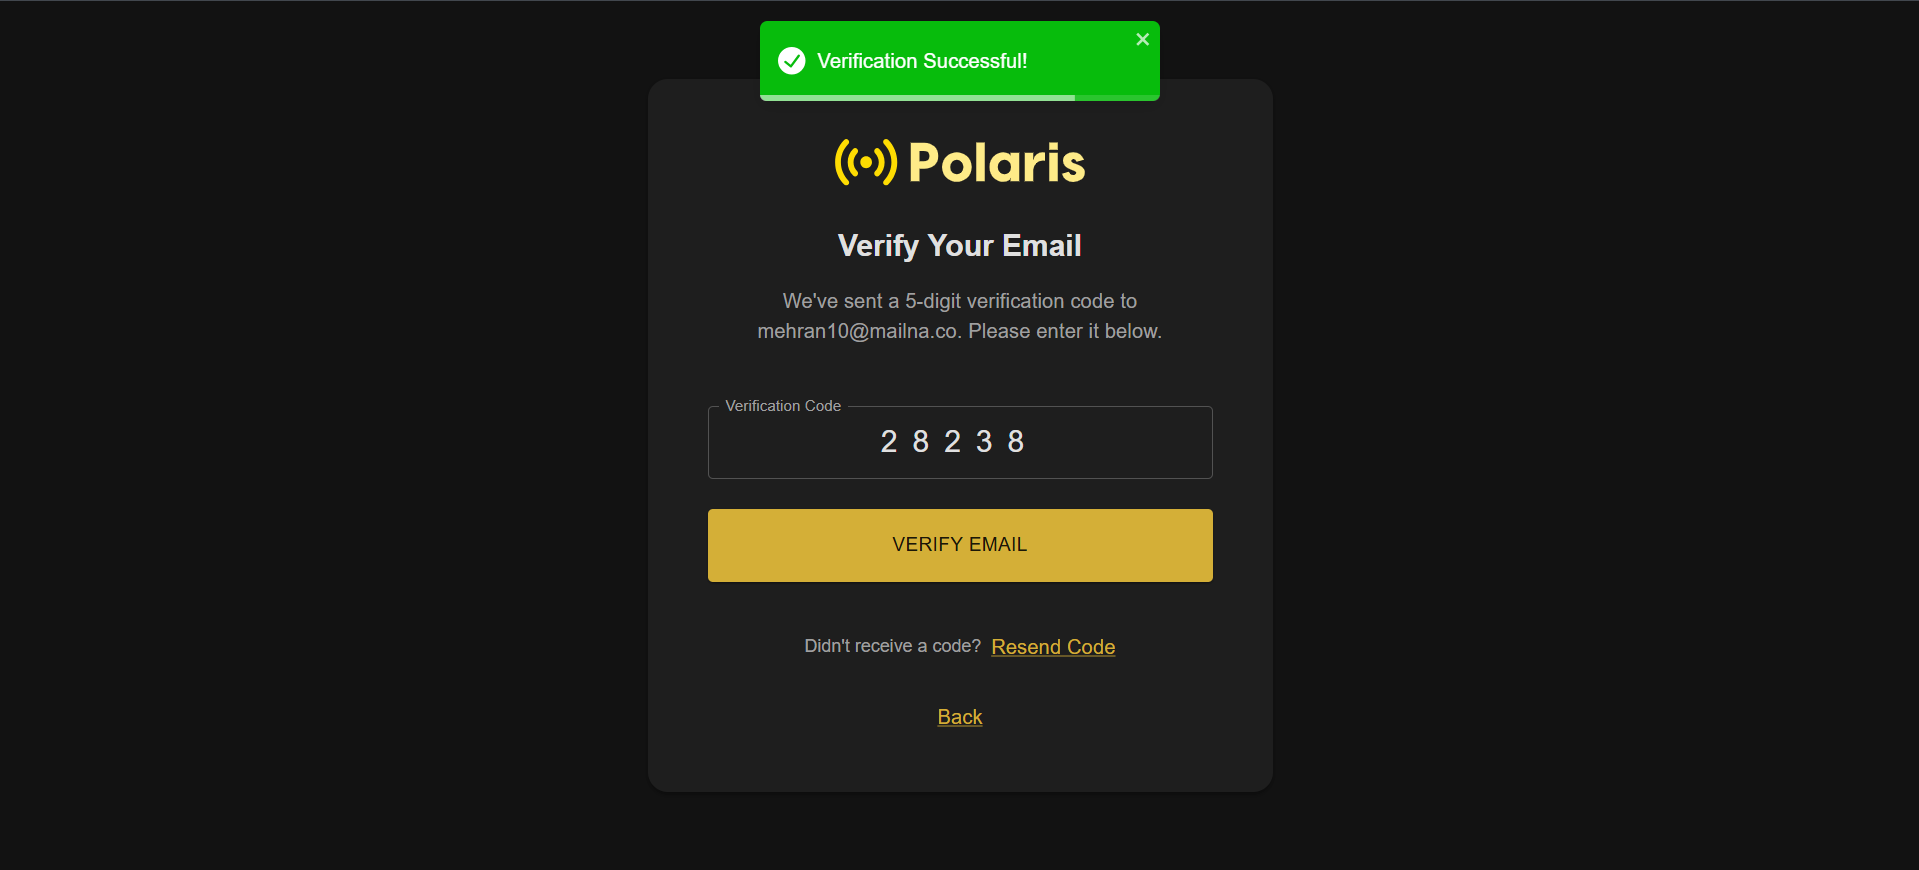
\includegraphics[width=\textwidth]{images/fr-verify-success.png}
    		\end{center}
    	\end{itemize}
    	
    	\item \textbf{ورود به حساب:}  
    	در صفحه ورود، پست الکترونیک یا شماره همراه و گذرواژه خود را وارد کرده و روی دکمه \lr{Login} کلیک کنید. در صورت وجود خطا (مانند رمز اشتباه)، پیام مناسب نمایش داده می‌شود. اگر ایمیل شما هنوز تأیید نشده باشد، سیستم شما را به صفحه تأیید هدایت خواهد کرد. در صورت موفقیت، پس از نمایش پیام زیر وارد داشبورد خواهید شد:
    	\begin{center}
    		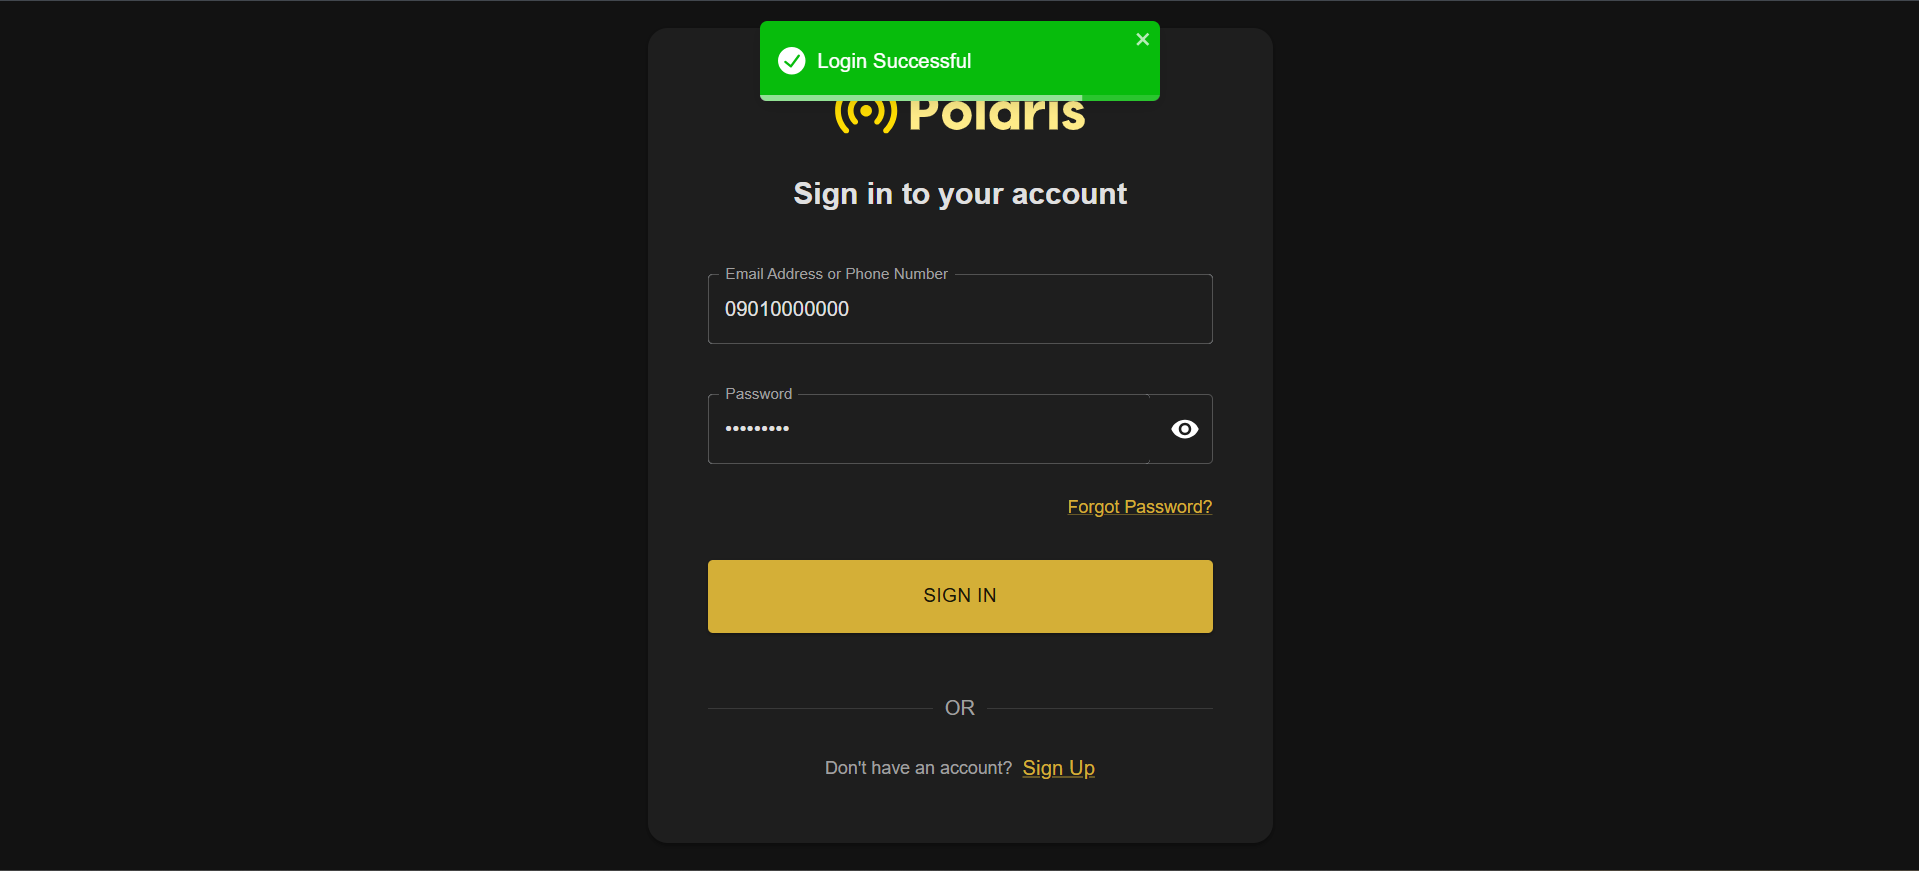
\includegraphics[width=\textwidth]{images/fr-login-success.png}
    	\end{center}
    	
    	\item \textbf{بازنشانی رمز عبور:}  
    	در صفحه ورود، با کلیک بر روی لینک \lr{Forgot Password?} به صفحه بازنشانی رمز عبور هدایت می‌شوید:
	    	\begin{center}
	    		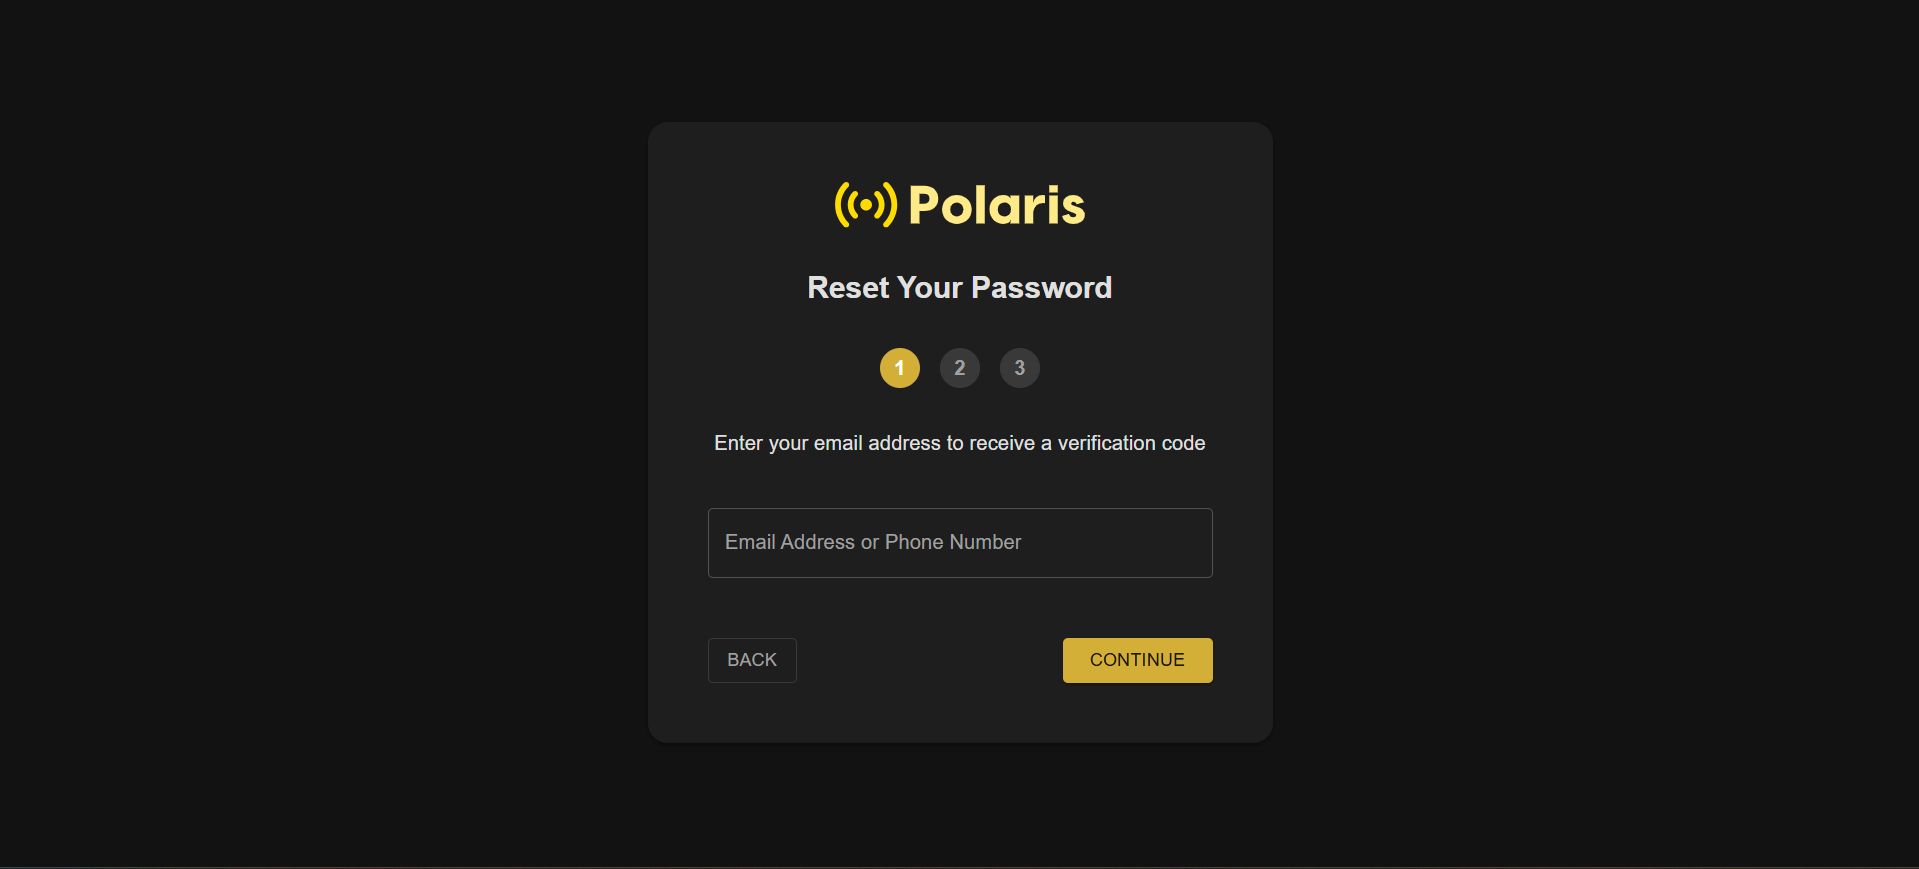
\includegraphics[width=\textwidth]{images/fr-reset-pass-empty.png}
	    	\end{center}
    	فرآیند بازنشانی رمز عبور شامل سه مرحله است:
    	\begin{itemize}
    		\item \textbf{مرحله ۱ (احراز هویت):}  
    		پست الکترونیک یا شماره همراه خود را وارد کرده و روی \lr{Send Code} کلیک کنید تا کد تأیید به ایمیل شما ارسال شود. در صورت موفقیت آمیز بودن این درخواست به مرحله بعدی می‌رویم و صفحه به صورت زیر خواهد شد:
    			\begin{center}
    				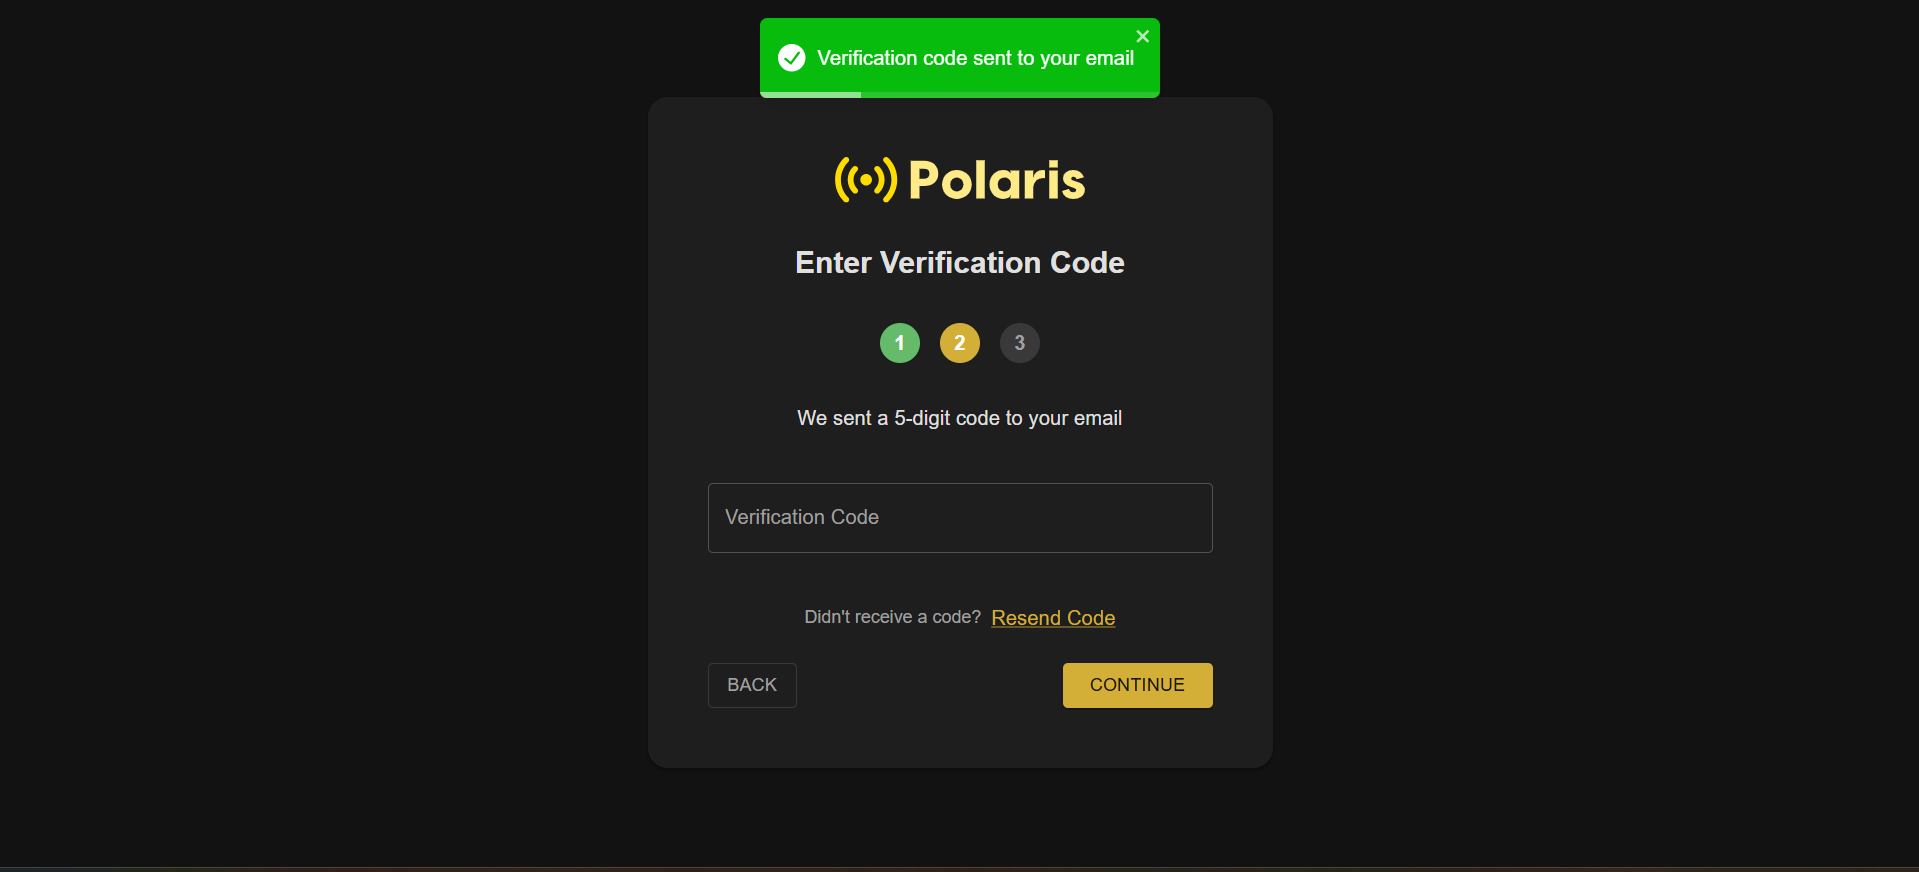
\includegraphics[width=\textwidth]{images/fr-verification-empty.png}
    			\end{center}
    		
    		\item \textbf{مرحله ۲ (تأیید):}  
    		در این مرحله کد ارسال‌شده به ایمیل را وارد کرده و روی \lr{Verify Code} کلیک کنید. امکان ارسال مجدد کد با \lr{Resend Code} یا بازگشت به مرحله قبل برای اصلاح اطلاعات  نیز وجود دارد. در صورت موفقیت آمیز بودن این درخواست صفحه به شکل زیر تغییر خواهد کرد:
    			\begin{center}
    				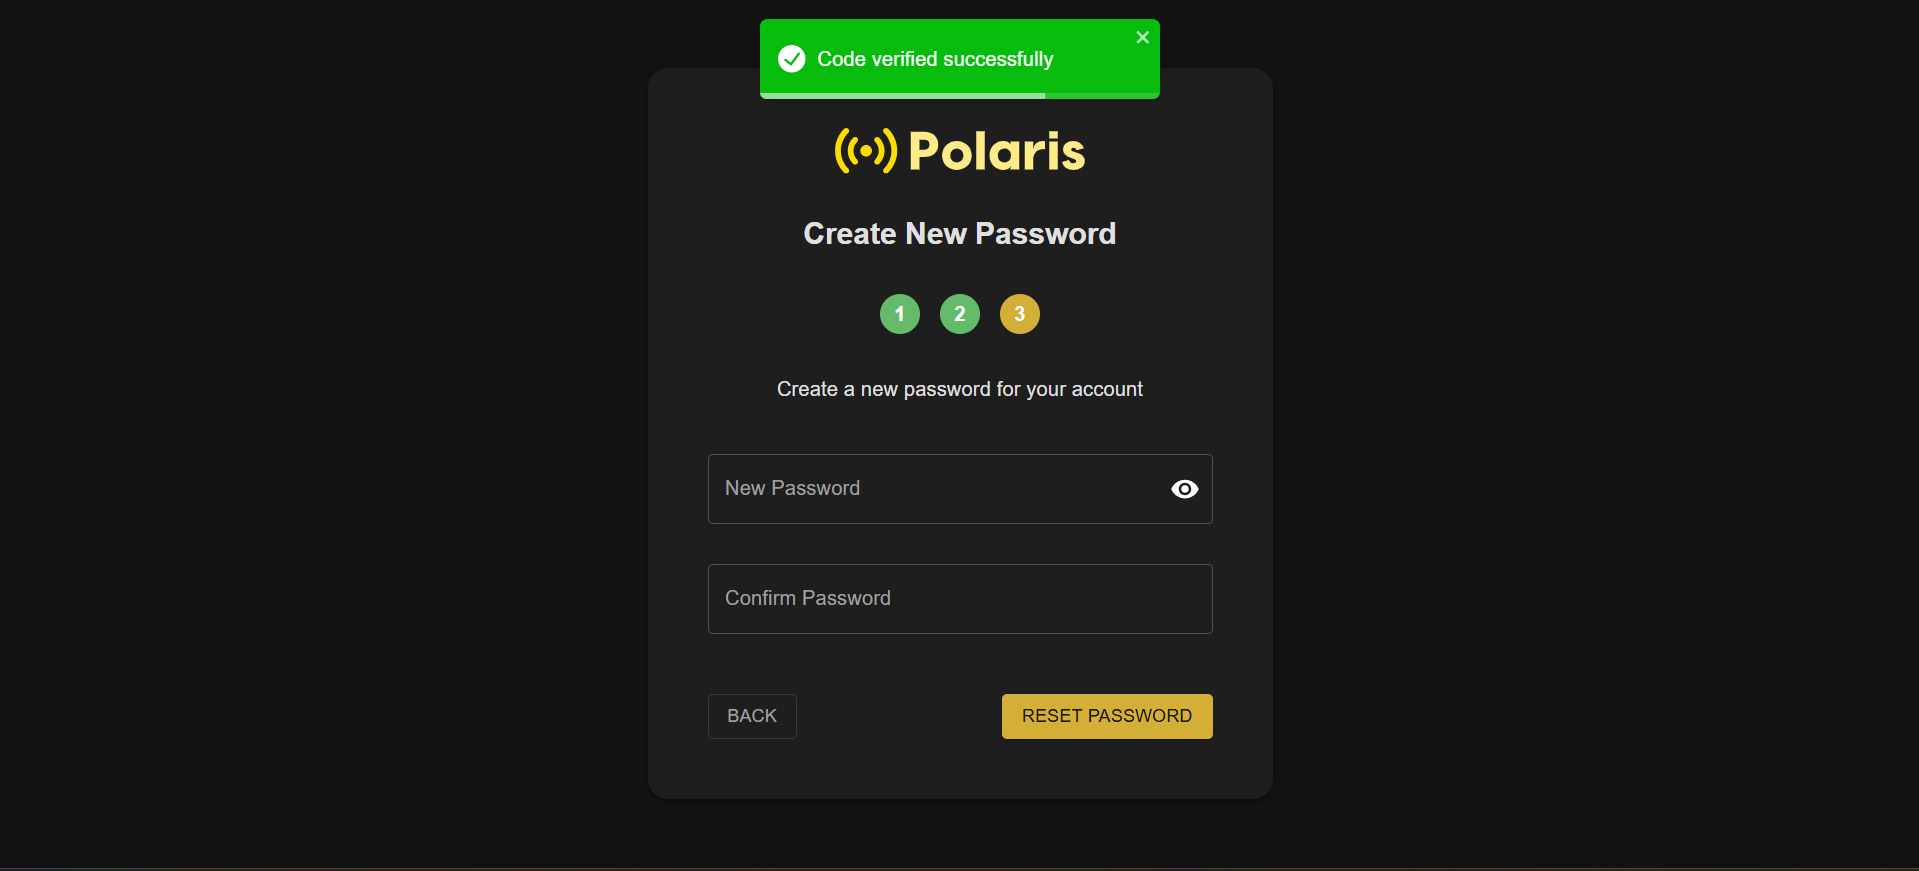
\includegraphics[width=\textwidth]{images/fr-new-pass-empty.png}
    			\end{center}
    		\item \textbf{مرحله ۳ (تغییر رمز عبور):}  
    		گذرواژه جدید (حداقل ۸ کاراکتر) را به همراه تکرار آن وارد کرده و روی \lr{Reset Password} کلیک کنید. پس از موفقیت، پیام زیر نمایش داده می‌شود و سپس به صفحه ورود منتقل خواهید شد:
		    	\begin{center}
		    		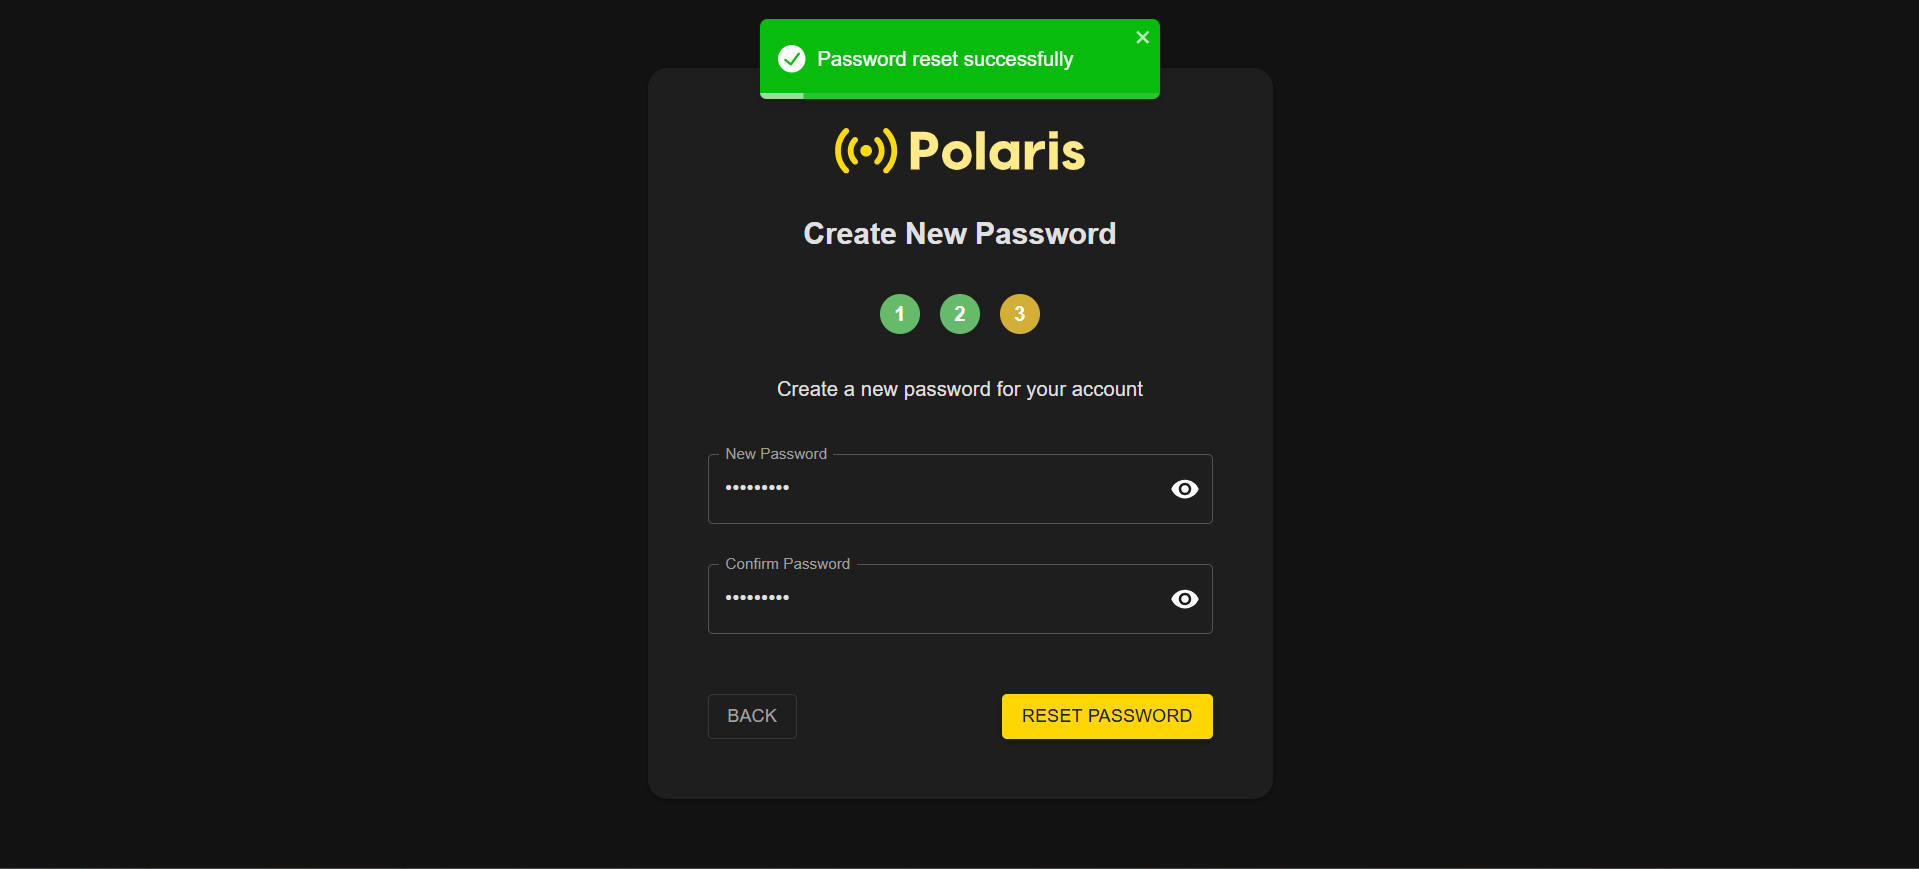
\includegraphics[width=\textwidth]{images/fr-new-pass-success.png}
		    	\end{center}
    	\end{itemize}
    \end{itemize}
    \section{بخش کاربری}
    \begin{itemize}
    	\item  مرور کلی داشبورد: پس از ورود به حساب در دفعه اول به دلیل نداشتن اطلاعات صفحه زیر را خواهید دید که فاقد اطلاعات می‌باشد:
    		\begin{center}
    			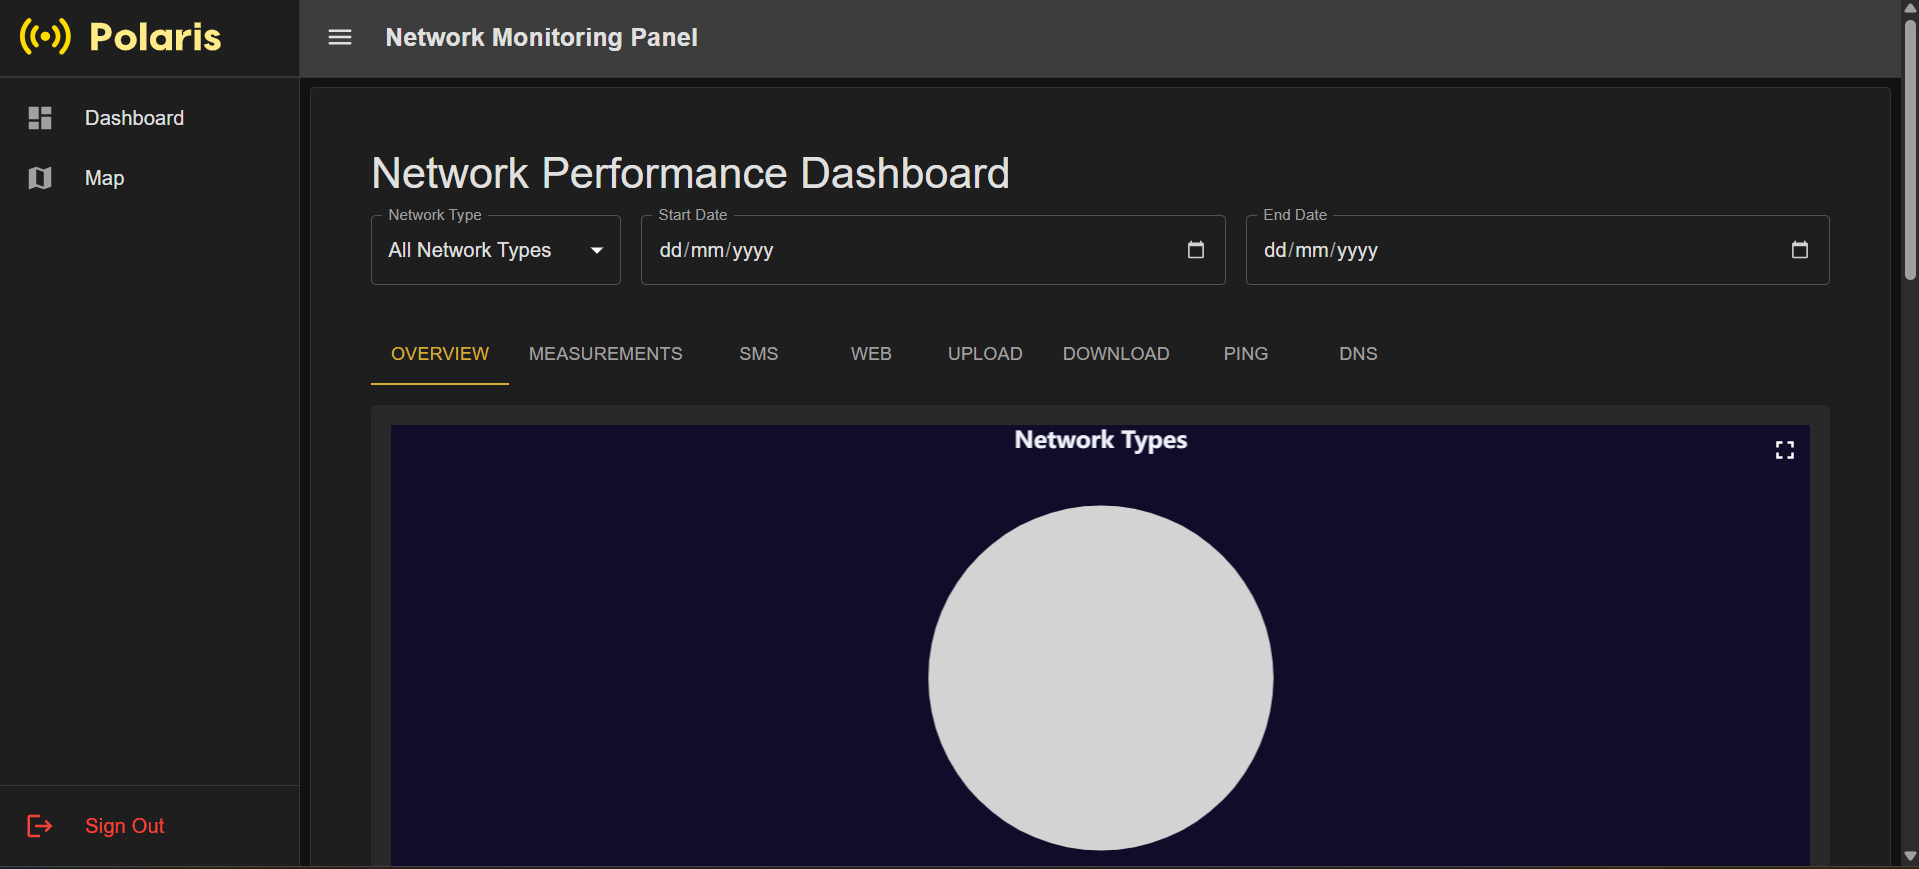
\includegraphics[width=\textwidth]{images/fr-dashboard-empty.png}
    		\end{center}
   		در صورت داشتن اطلاعات از پیش داشبورد به صورت زیر خواهد بود:
	   		\begin{center}
	   			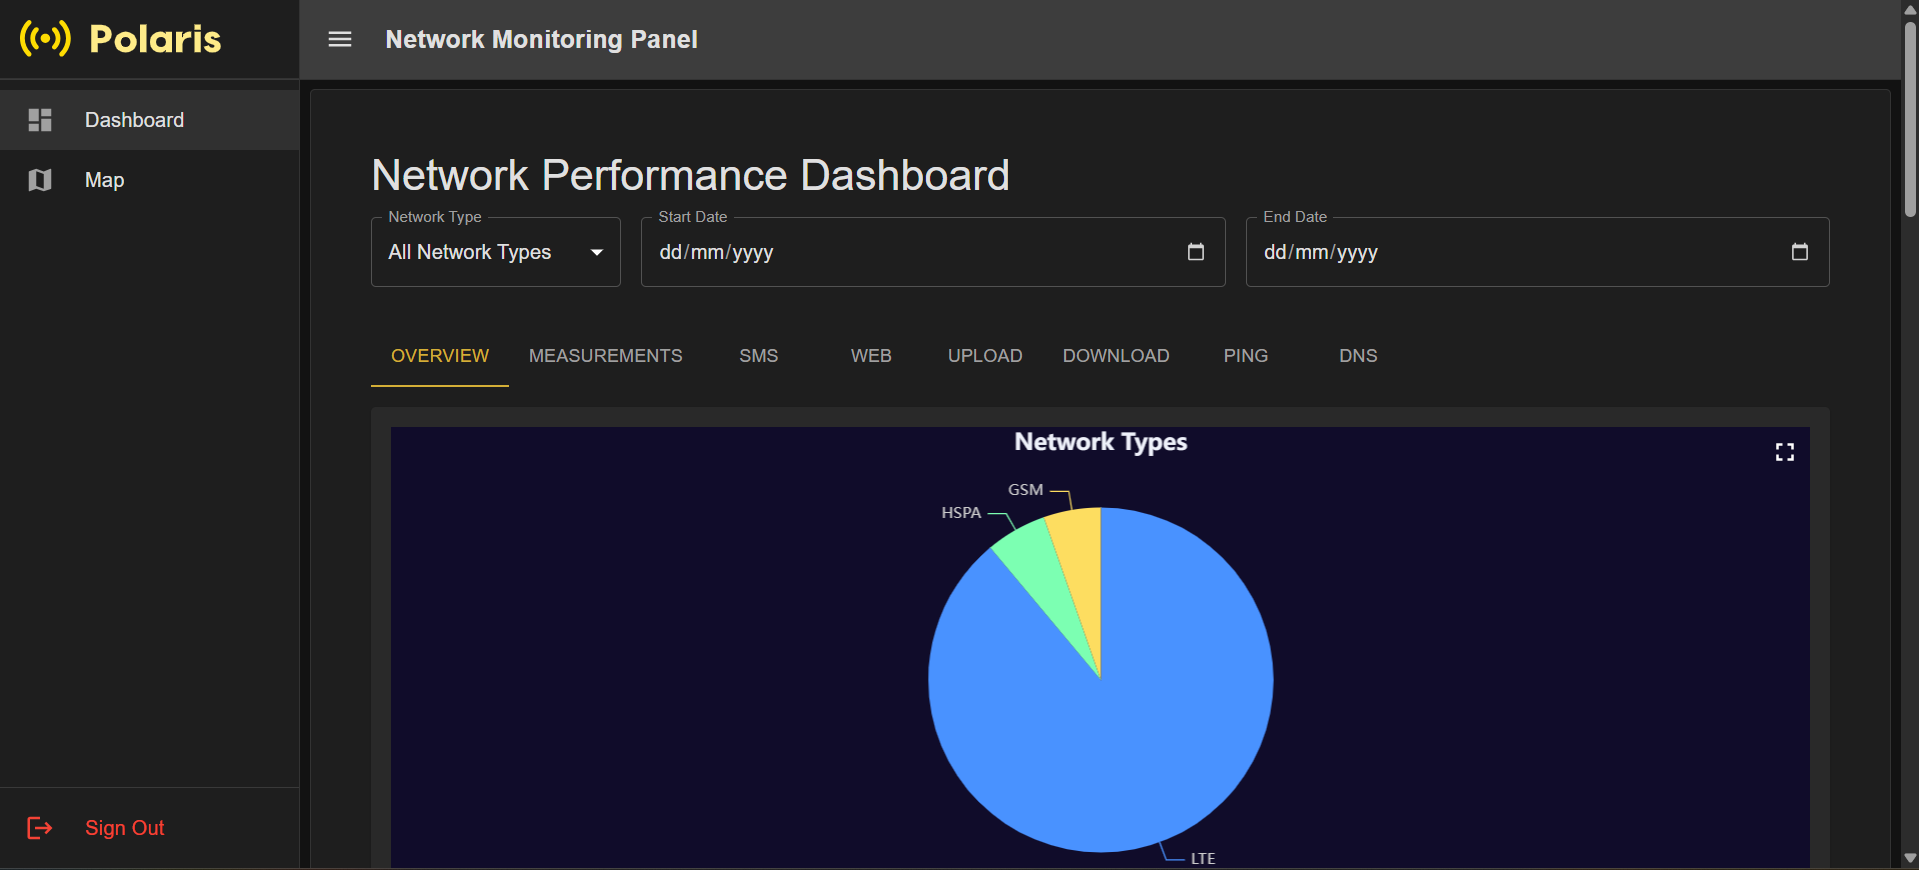
\includegraphics[width=\textwidth]{images/fr-dashboard-filled.png}
	   		\end{center}
	   	با کلیک بر روی آیکن سه خط در بالای سمت چپ که در تصویر زیر با کادر قرمز مشخص شده است نمای کناری سایت تا حدی پنهان می‌شود تا محتوای اصلی سایت بهتر نمایش داده شود:
	   		\begin{center}
				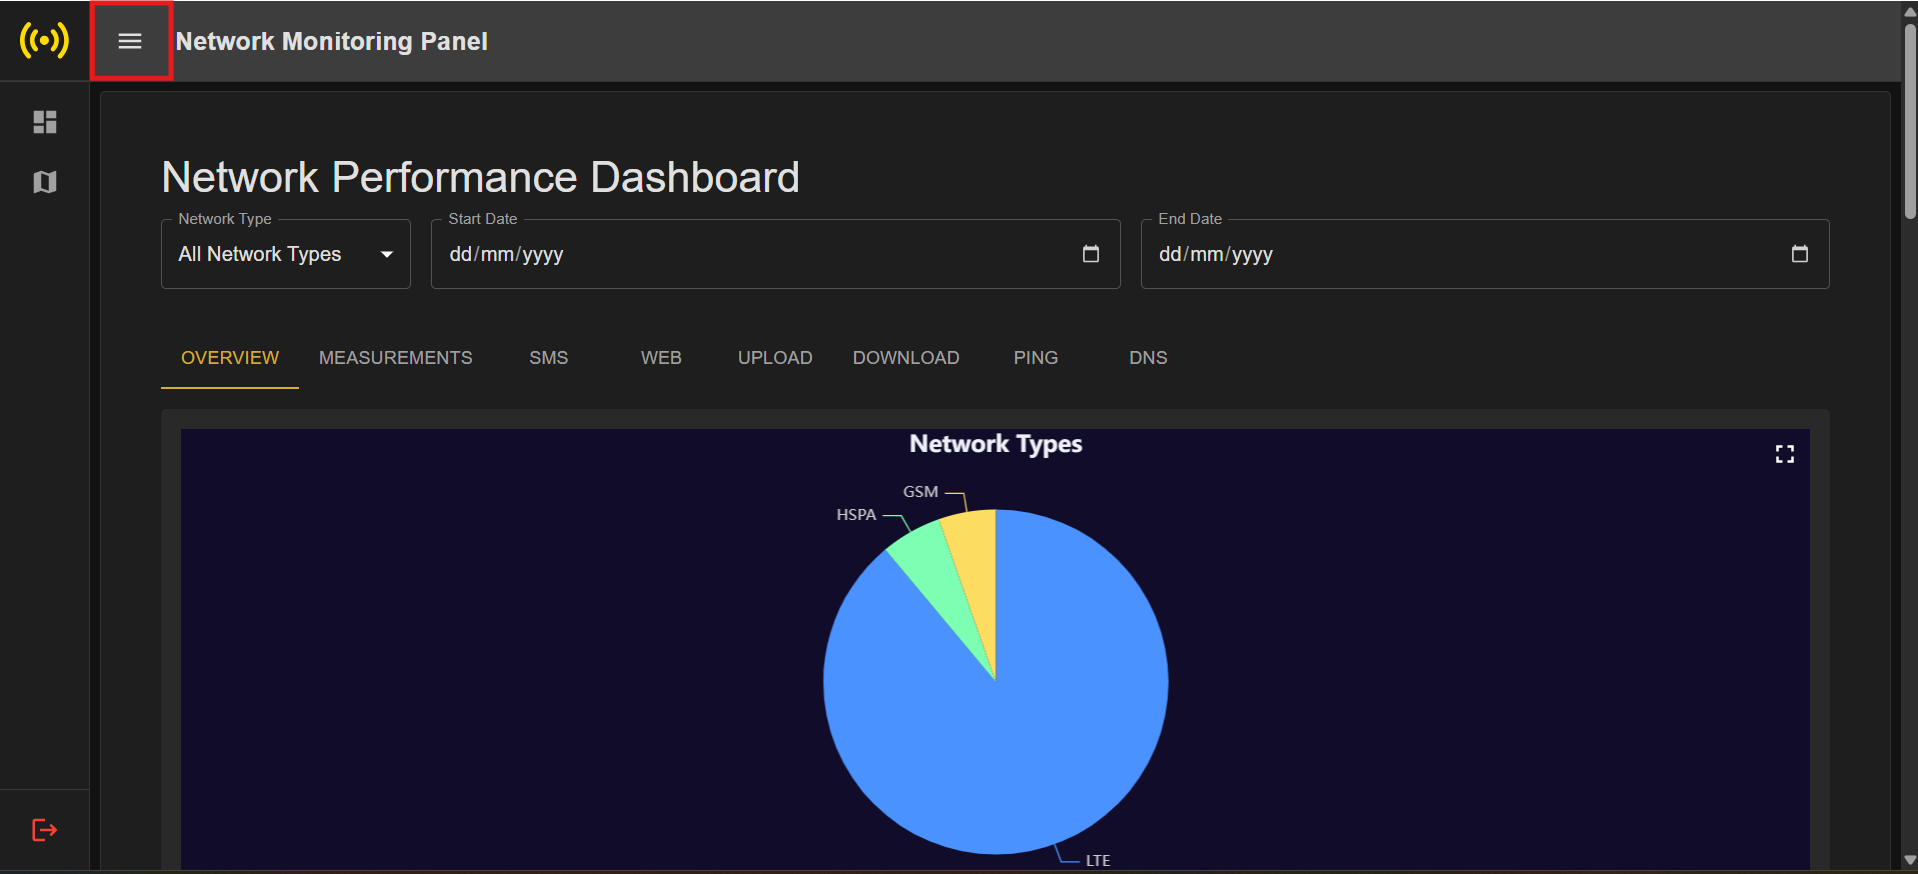
\includegraphics[width=\textwidth]{images/fr-dashboard-without-sidebar.png}
			\end{center}	   		
		در داشبورد وب‌سایت این امکان مقدور گردیده است که داده‌ها بر اساس نوع شبکه پیکربندی شود:
			\begin{center}
				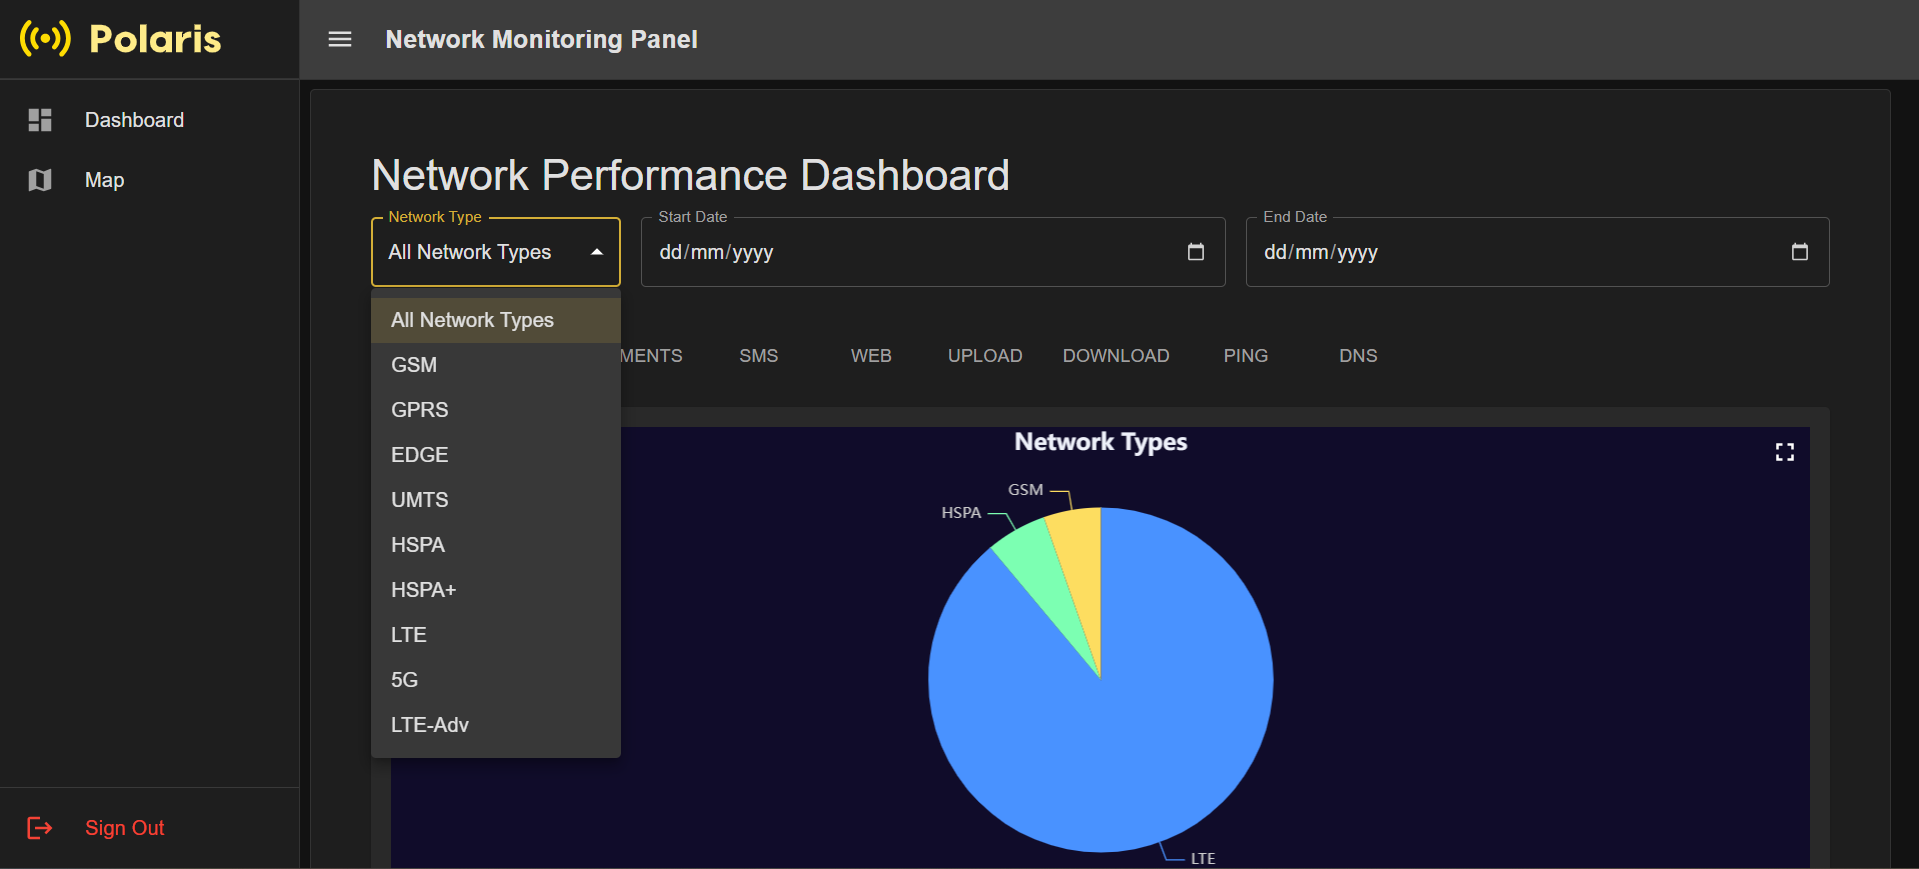
\includegraphics[width=\textwidth]{images/fr-filters-network.png}
			\end{center}	   		
   		در داشبورد وب‌سایت این امکان مقدور گردیده است که داده‌ها بر اساس تاریخ شروع و تاریخ پایان نیز پیکربندی شود:
	   		\begin{center}
	   			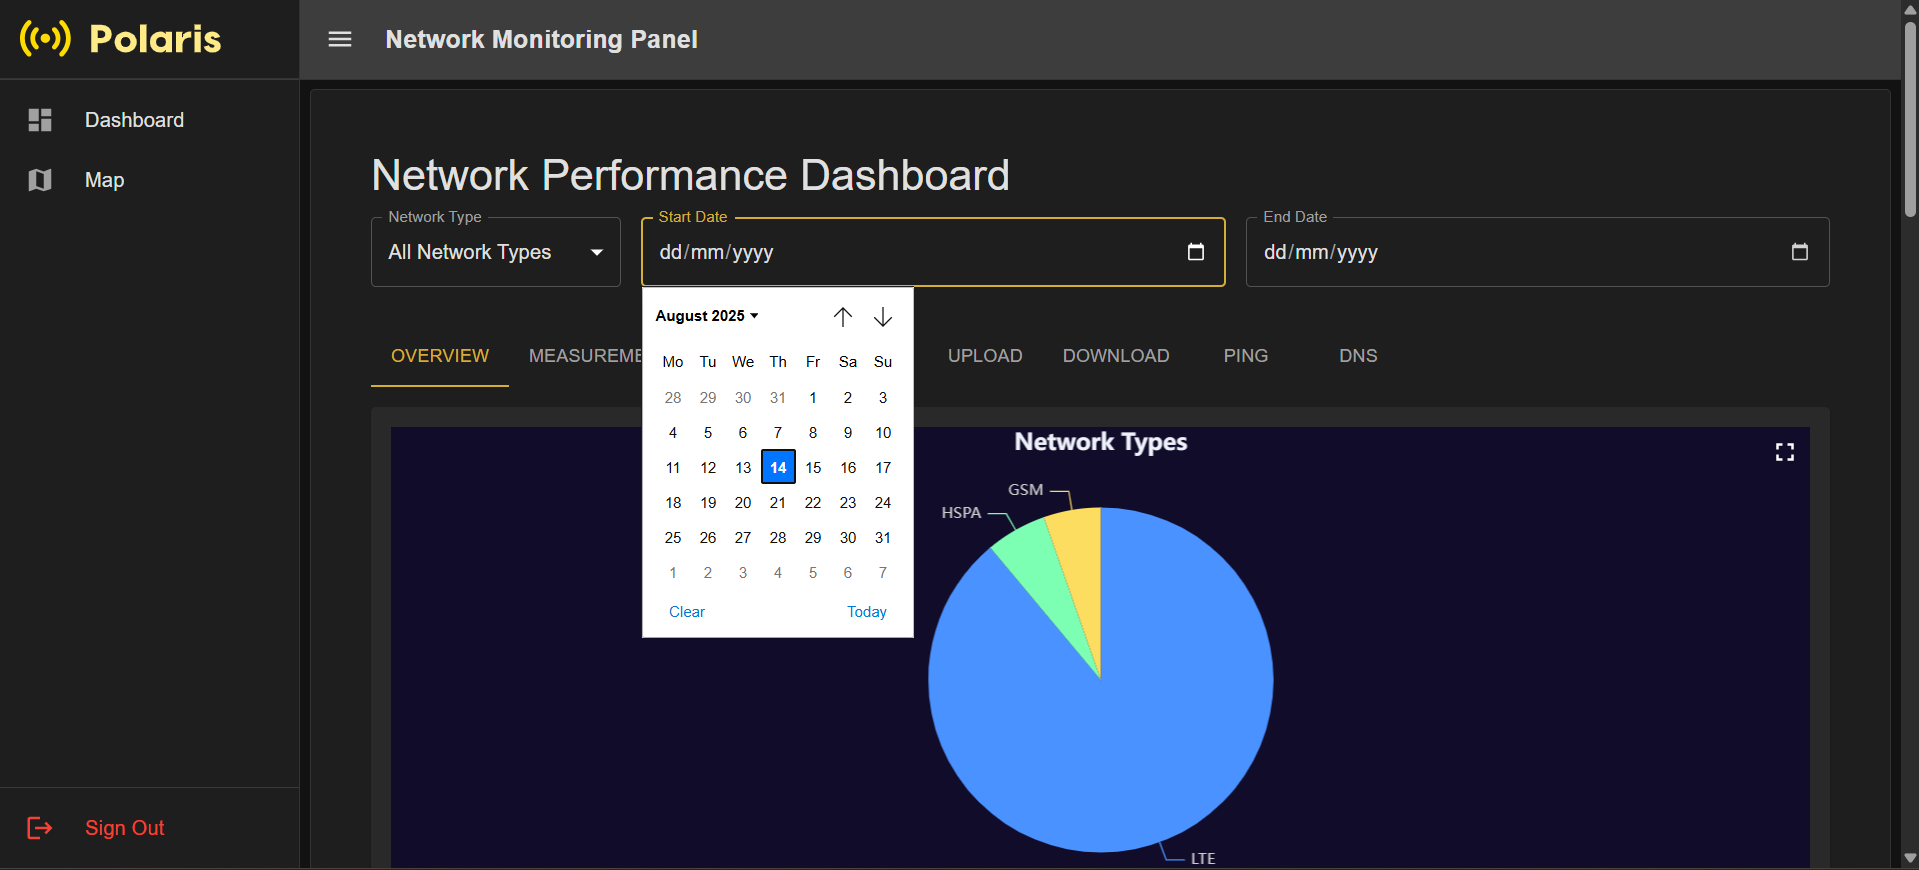
\includegraphics[width=\textwidth]{images/fr-filters-start-date.png}
	   			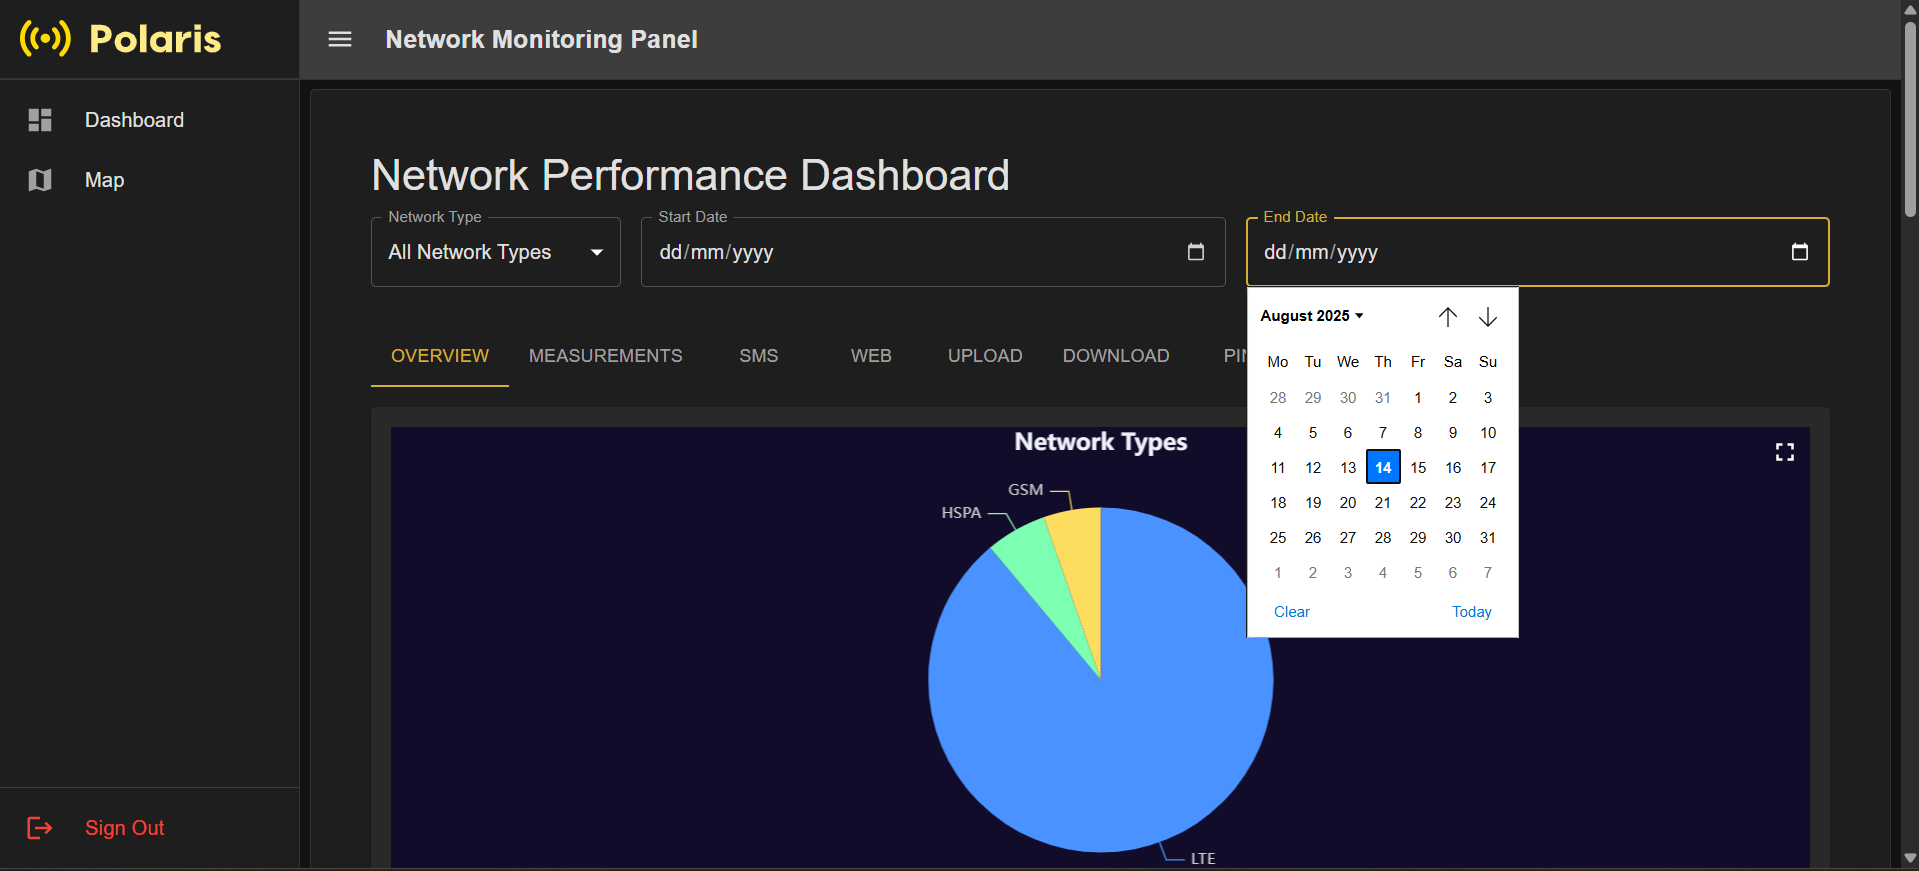
\includegraphics[width=\textwidth]{images/fr-filters-end-date.png}
	   		\end{center}
   		
   		داشبورد در بخش‌های متفاوتی از جمله Overview(که داده‌ها را در یک نگاه نمایش می‌دهد) و Measurements(که اندازه‌گیری‌های غیر از تست‌های تعریف شده توسط کاربر را نمایش می‌دهد) تقسیم شده است و دیگر بخش‌ها مختص تست‌های تعریف شده توسط کاربر است.
   		لازم به ذکر است که هر نمودار دارای دکمه‌ای در گوشۀ بالا سمت راست خود دارد که در تصویر زیر با کادر قرمز رنگ مشخص شده است و این امکان را می‌دهد که نمودار به صورت کامل صفحه را می‌پوشاند و باعث مشاهده بهتر آن می‌شود:
	   		\begin{center}
	   			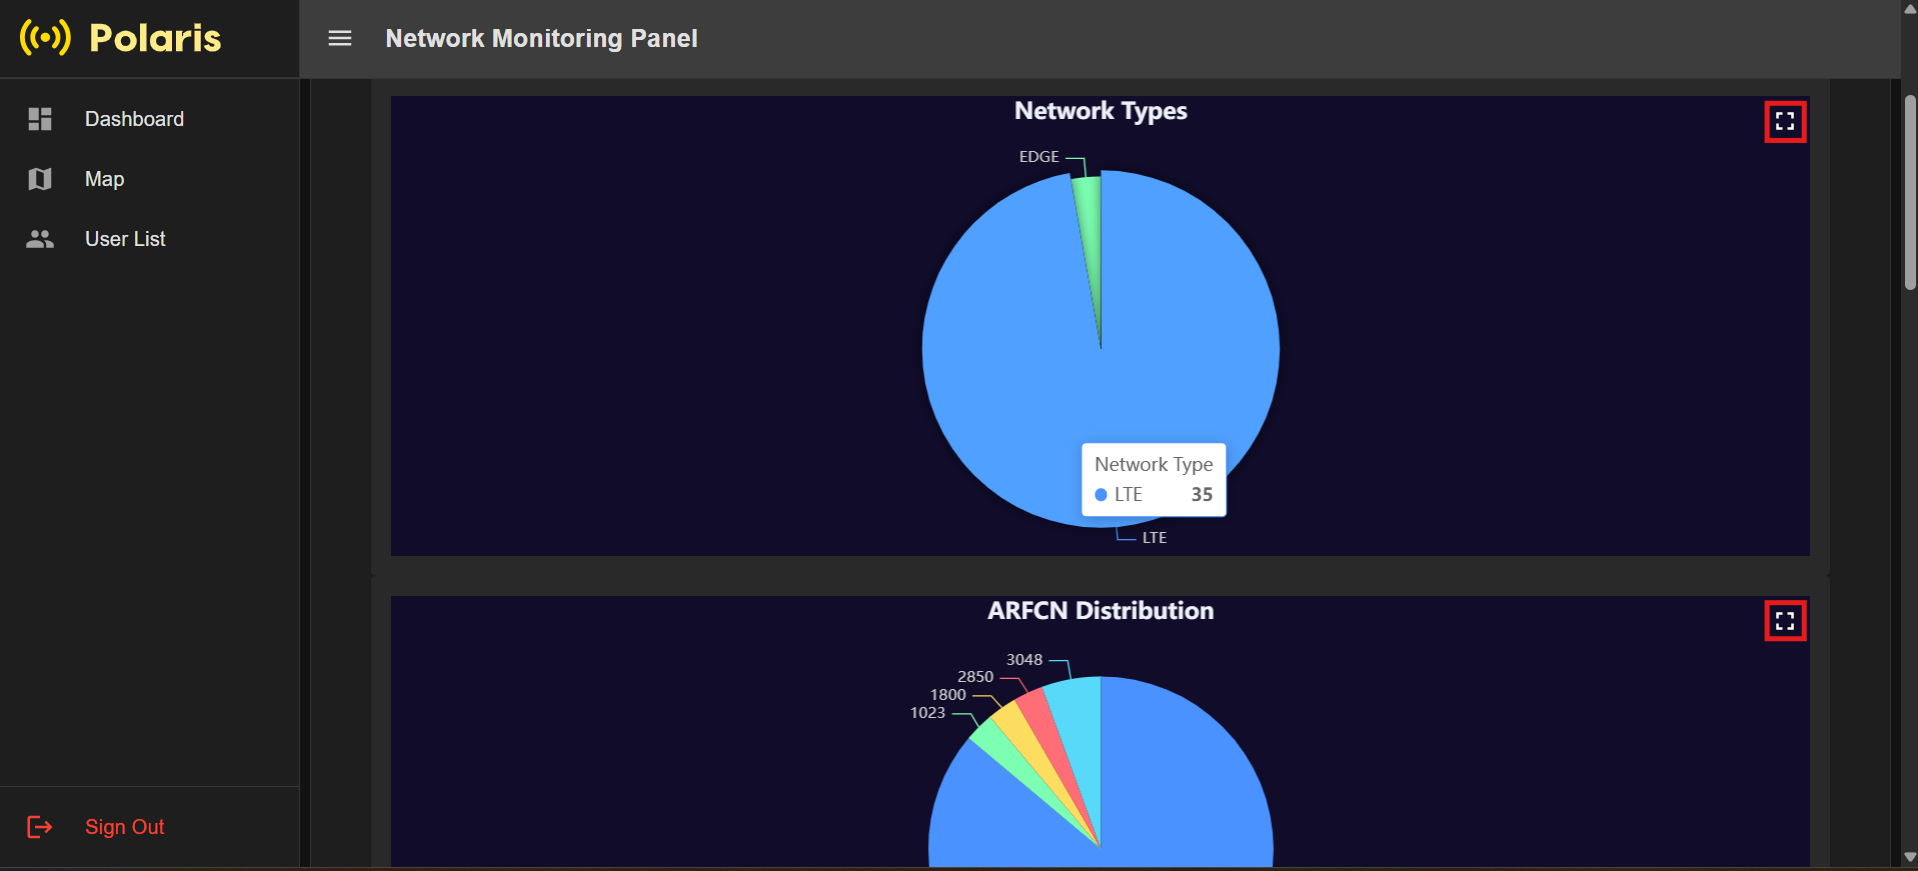
\includegraphics[width=\textwidth]{images/fr-chart-minimize.png}
	   		\end{center}
   		در این حالت با زدن روی این دکمه صفحه به صورت زیر خواهد شد که با انتخاب دکمه ضربدر که با کادر قرمز رنگ مشخص شده است صفحه به حالت قبلی بر‌میگردد:
	   		\begin{center}
				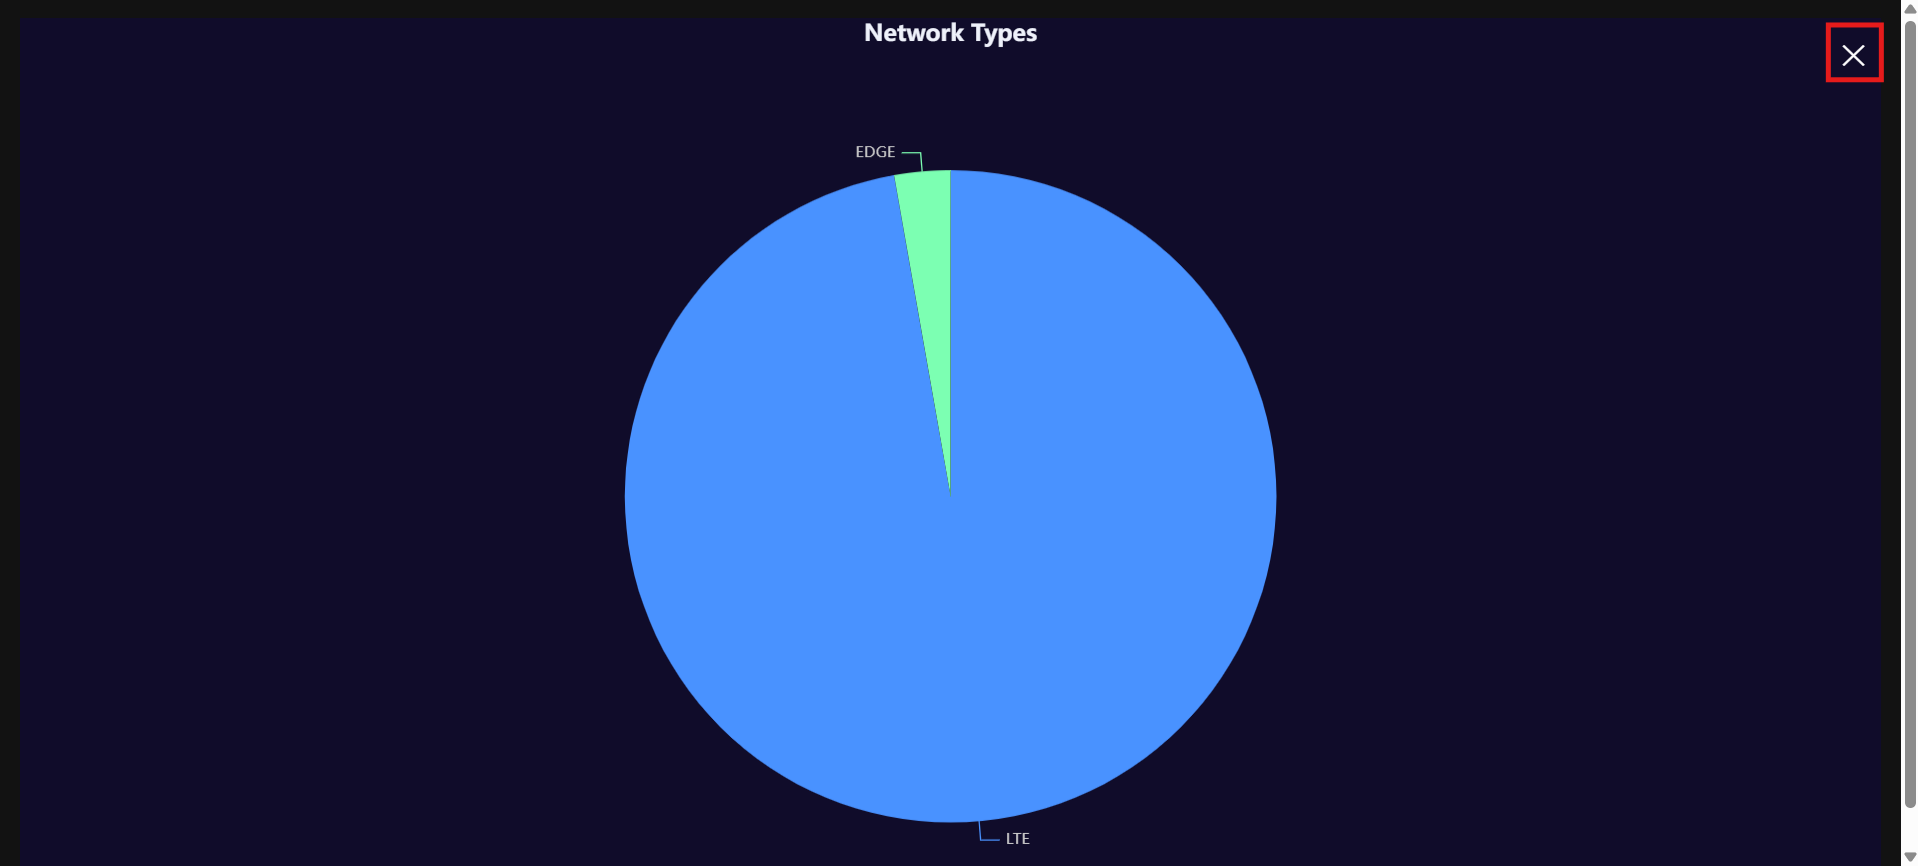
\includegraphics[width=\textwidth]{images/fr-chart-maximize.png}
			\end{center}
		در انتهای هر بخش داشبورد یک جدول وجود دارد که امکان مشاهده همه اطلاعات را در یک نگاه می‌دهد. همجنین قابلیت استخراج اطلاعات به صورت csv و kml نیز آمده است که با کلیک روی دکمه آن(که با کادر قرمز رنگ مشخص شده است) فایل با فرمت موردنظر دانلود می‌شود:
			\begin{center}
				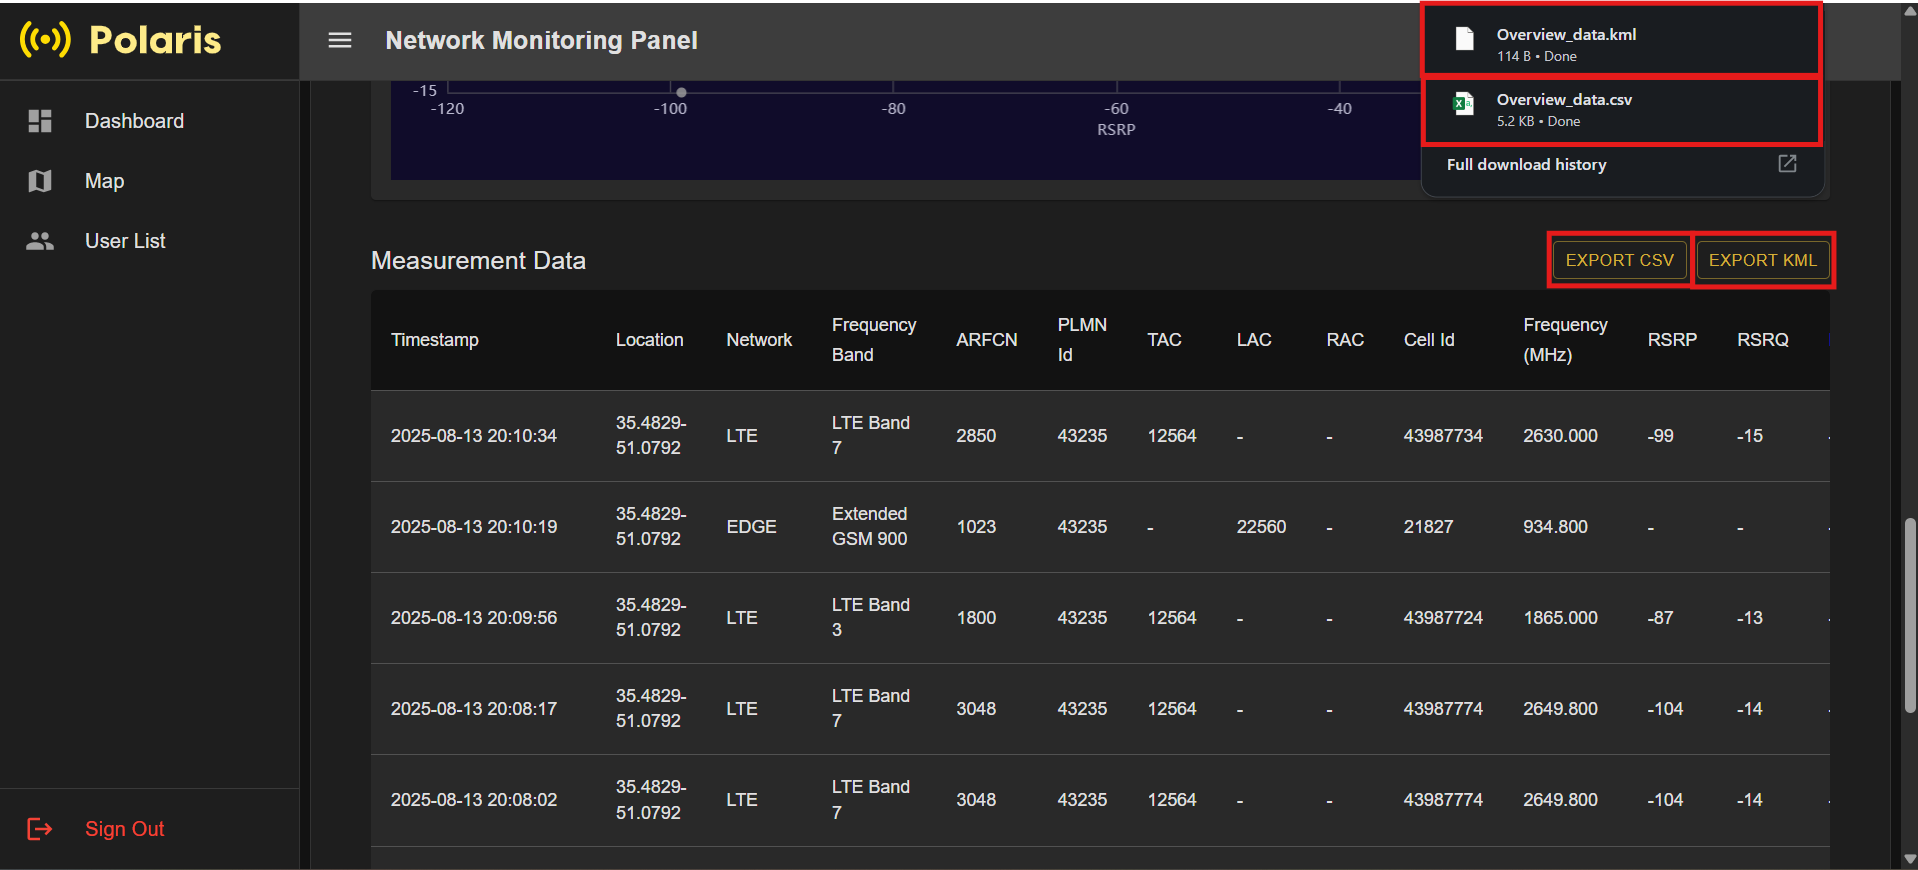
\includegraphics[width=\textwidth]{images/fr-table-export.png}
			\end{center}
   		از آنجایی که احتمالا هر کاربر تعداد زیادی داده خواهد داشت هر جدول تعداد محدودی از داده‌ها را نمایش می‌دهد که می‌توان آن را تغییر داد. همچنین می‌توان بین داده‌های هر صفحه جابه‌جا شد و انتهای جدول نمایش می‌دهد که این اطلاعات کدامین ردیف‌های اطلاعات کاربر می‌باشند و کاربر چه تعداد اطلاعات دارد:
   			\begin{center}
   				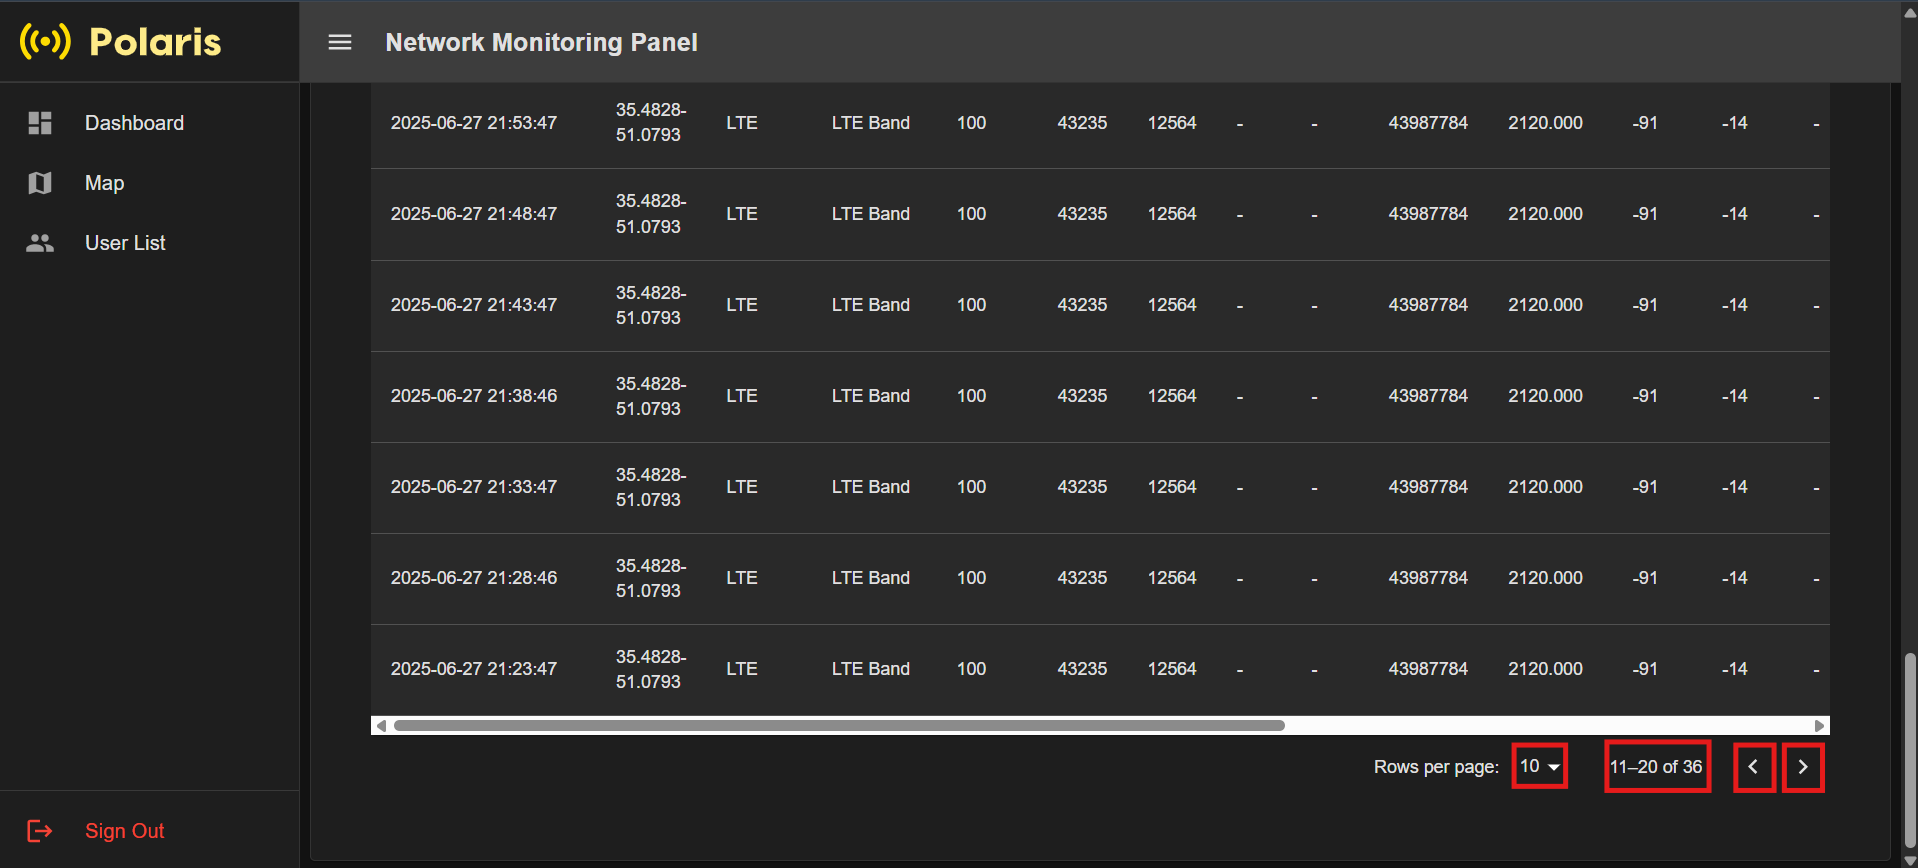
\includegraphics[width=\textwidth]{images/fr-table-pagination.png}
   			\end{center}
    	\item  استفاده از نقشه: توضیح نحوه تعامل با ویژگی نقشه.
    	\item  خروج از سیستم: می‌توان از طریق کلیک بر روی دکمه \lr{Sign Out} که در تصویر زیر نیز مشخص شده است از حساب کاربری خود خروج پیدا کرد:
    		\begin{center}
    			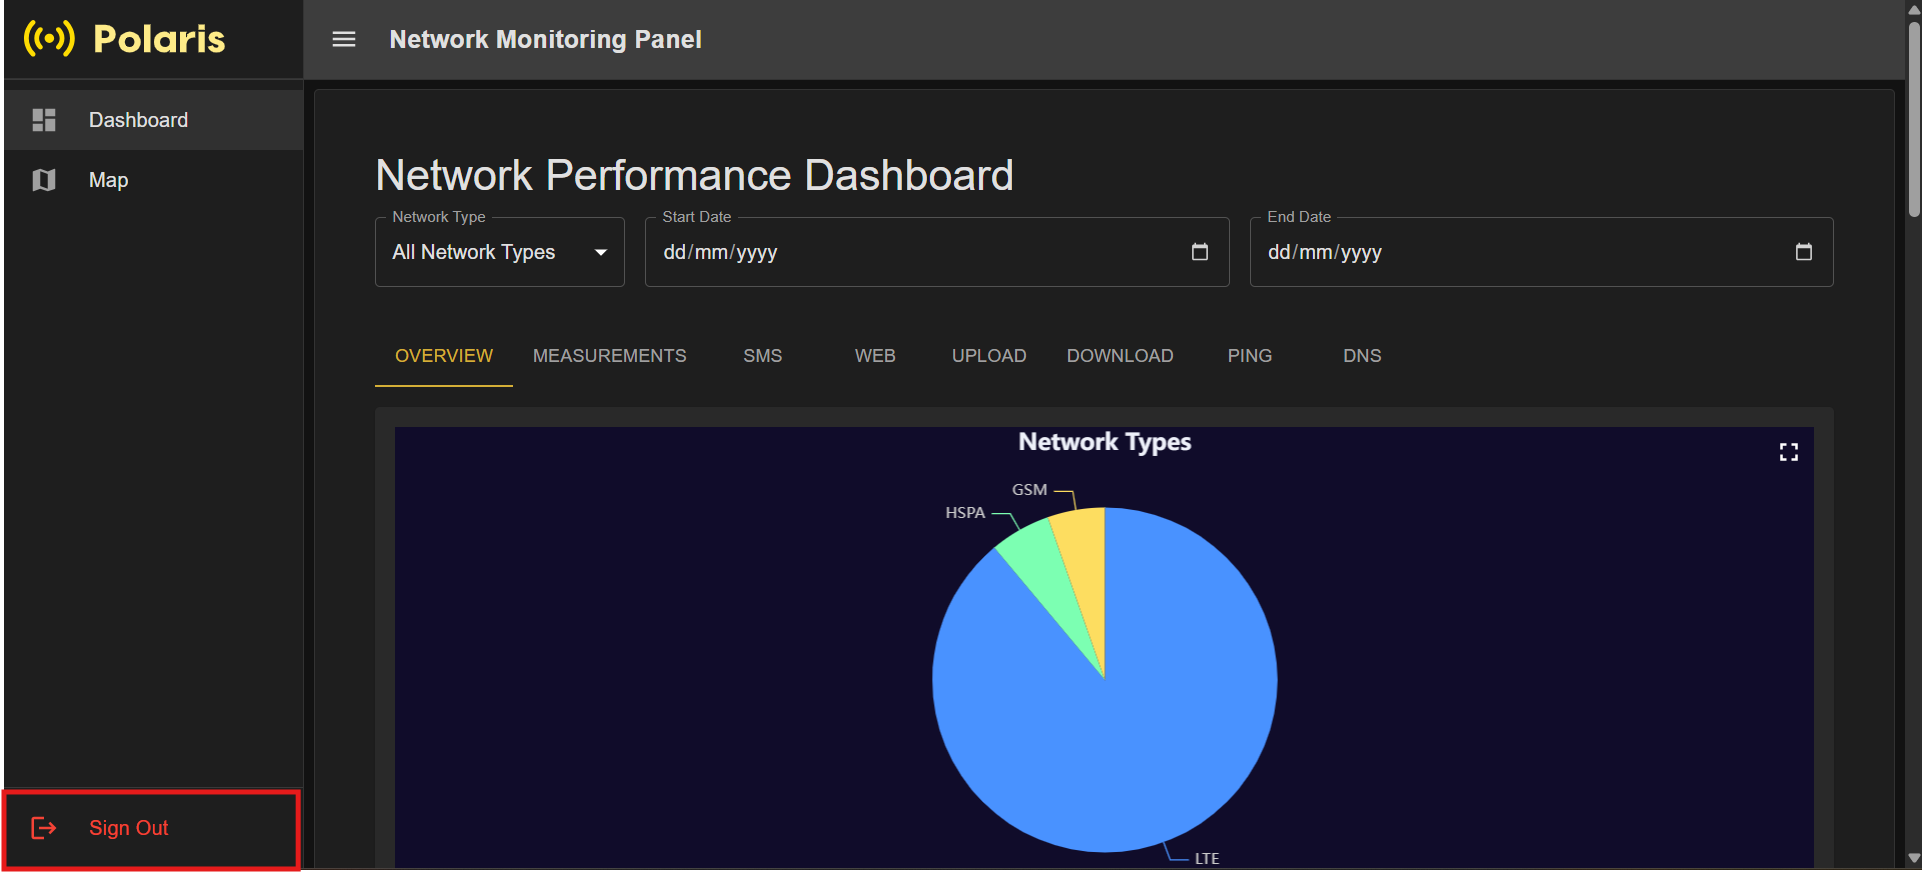
\includegraphics[width=\textwidth]{images/fr-signout.png}
    		\end{center}
    \end{itemize}
    \section{ویژگی‌های مدیر}
    \begin{itemize}
    	\item  لیست کاربران: فردی که توسط سرور به عنوان ادمین انتخاب شود می‌تواند لیست همه کاربران غیر ادمین به همراه اطلاعات آن ها را مشاهده کند که به صورت زیر است:
    		\begin{center}
    			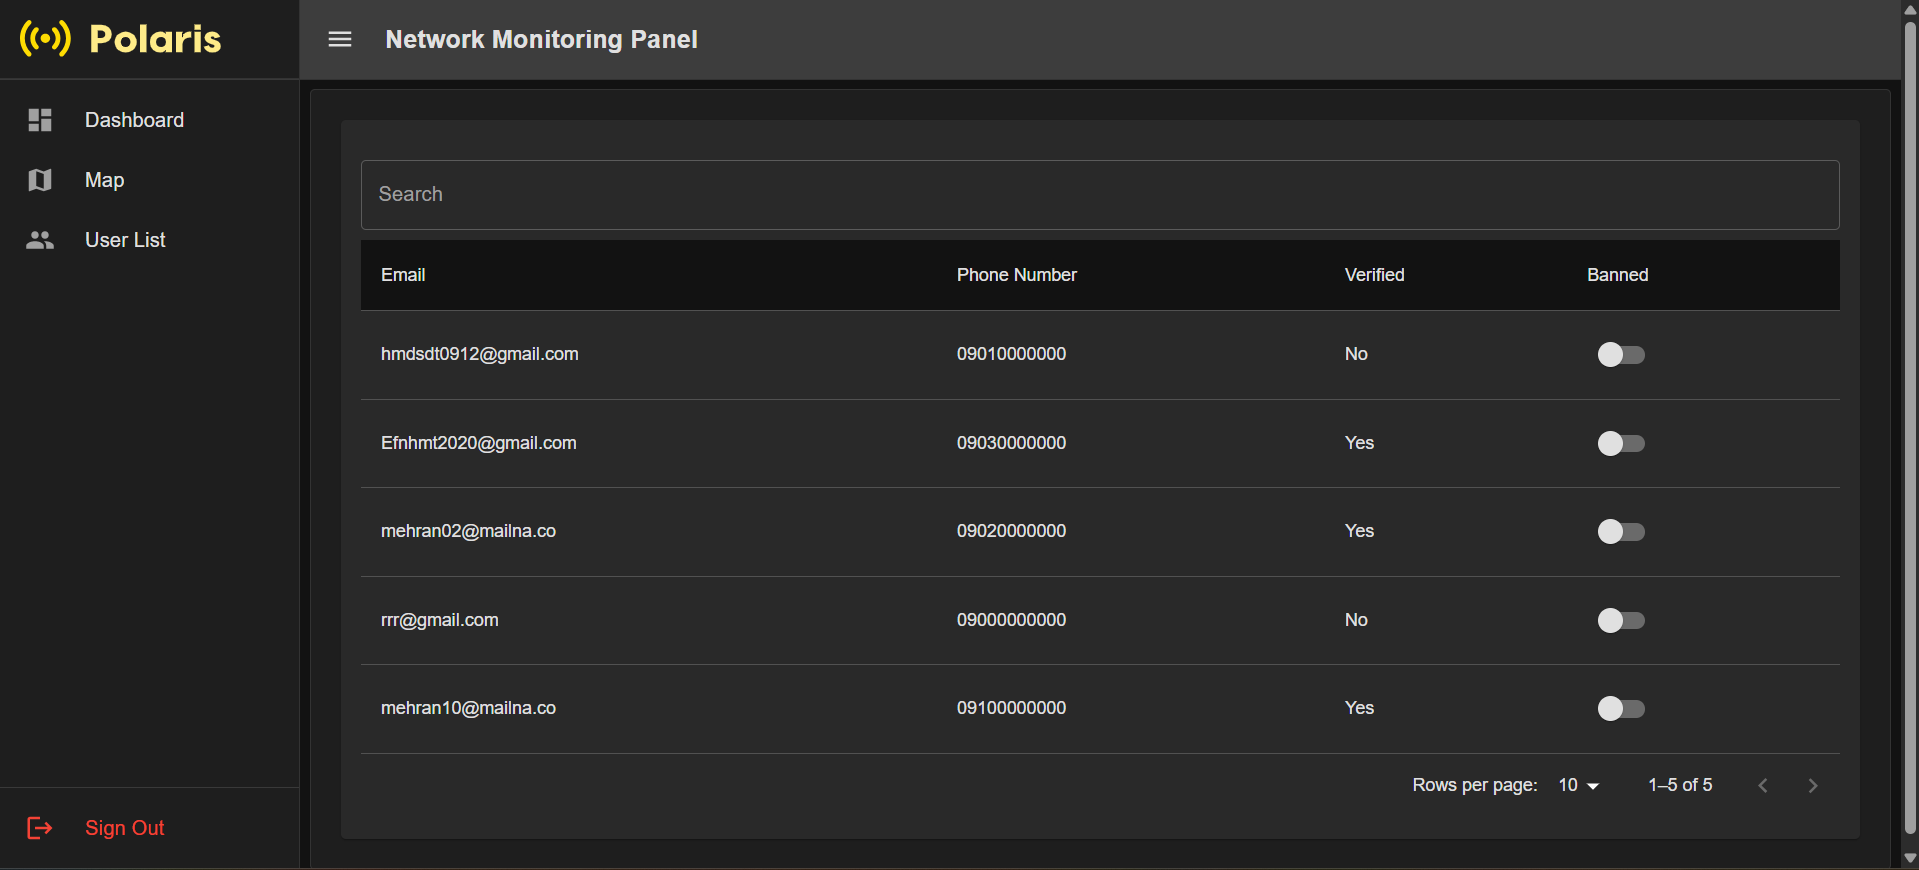
\includegraphics[width=\textwidth]{images/fr-userlist.png}
    		\end{center}
    	این امکان به مدیر داده شده است که بتواند یک کاربر را به حالت تعلیق در بیاورد به این صورت که در ستون Banned می‌تواند سوییچ را روشن و خاموش کند که در صورت روشن کردن کاربر موردنظر دیگر امکان ورود به حساب خود را ندارد و در صورت خاموش بودن روند ورود کاربر به حساب خود به صورت عادی خواهد بود:
    		\begin{center}
    			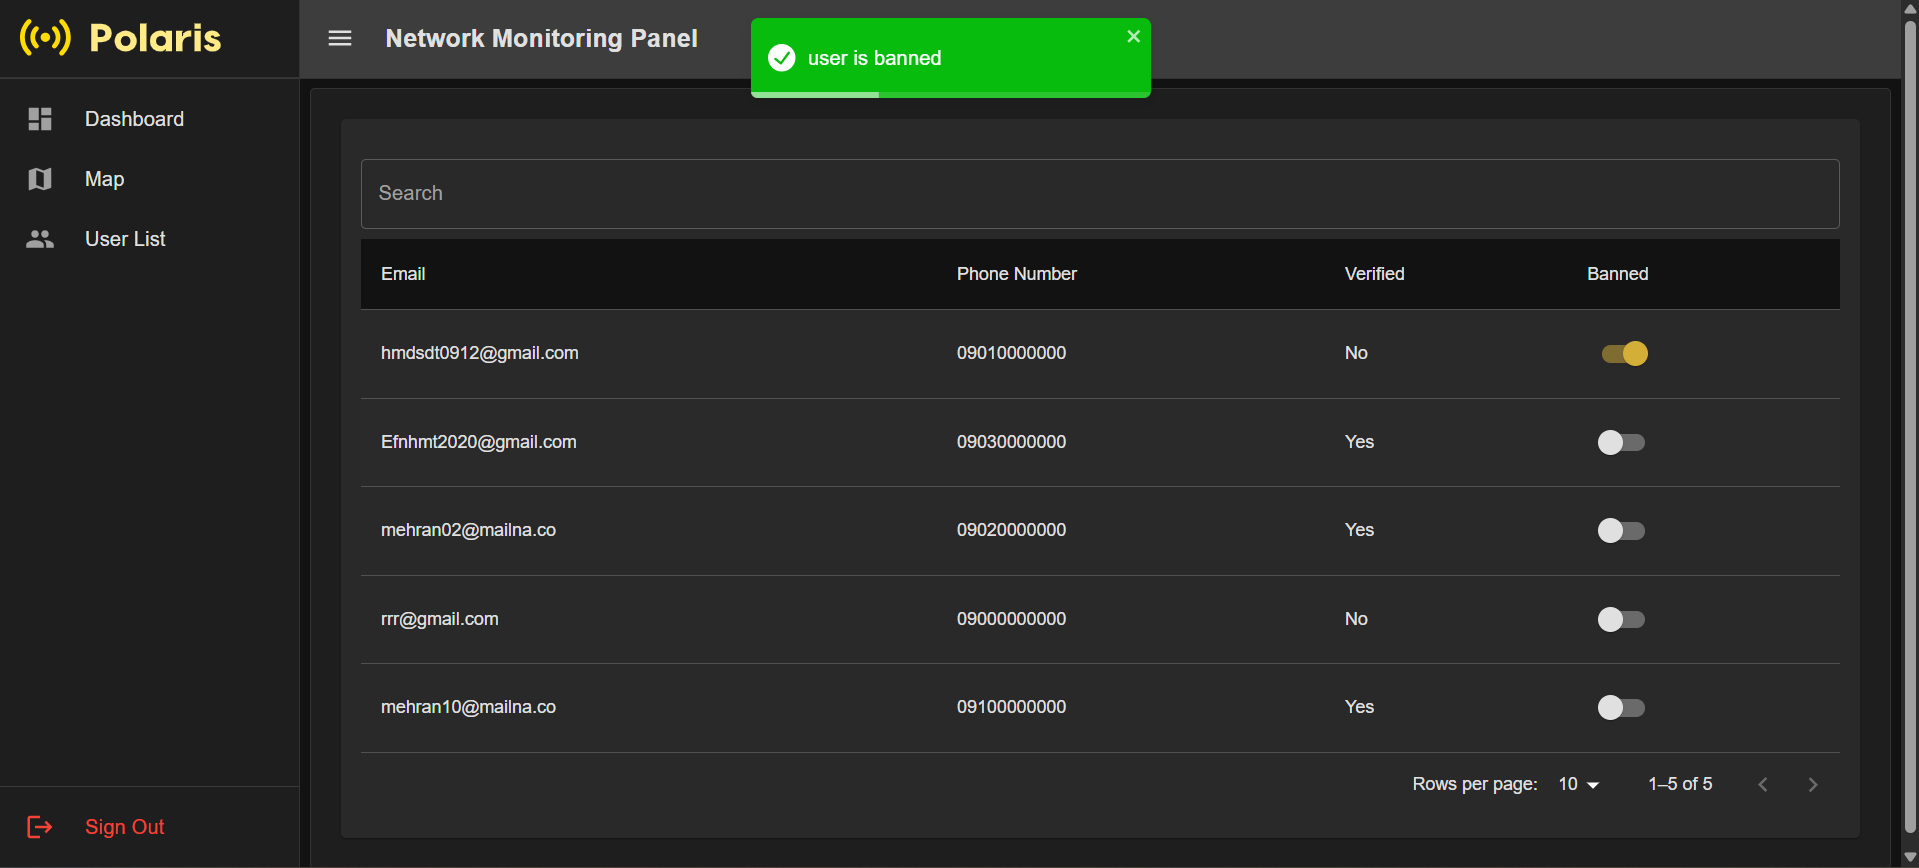
\includegraphics[width=\textwidth]{images/fr-userlist-ban.png}
    			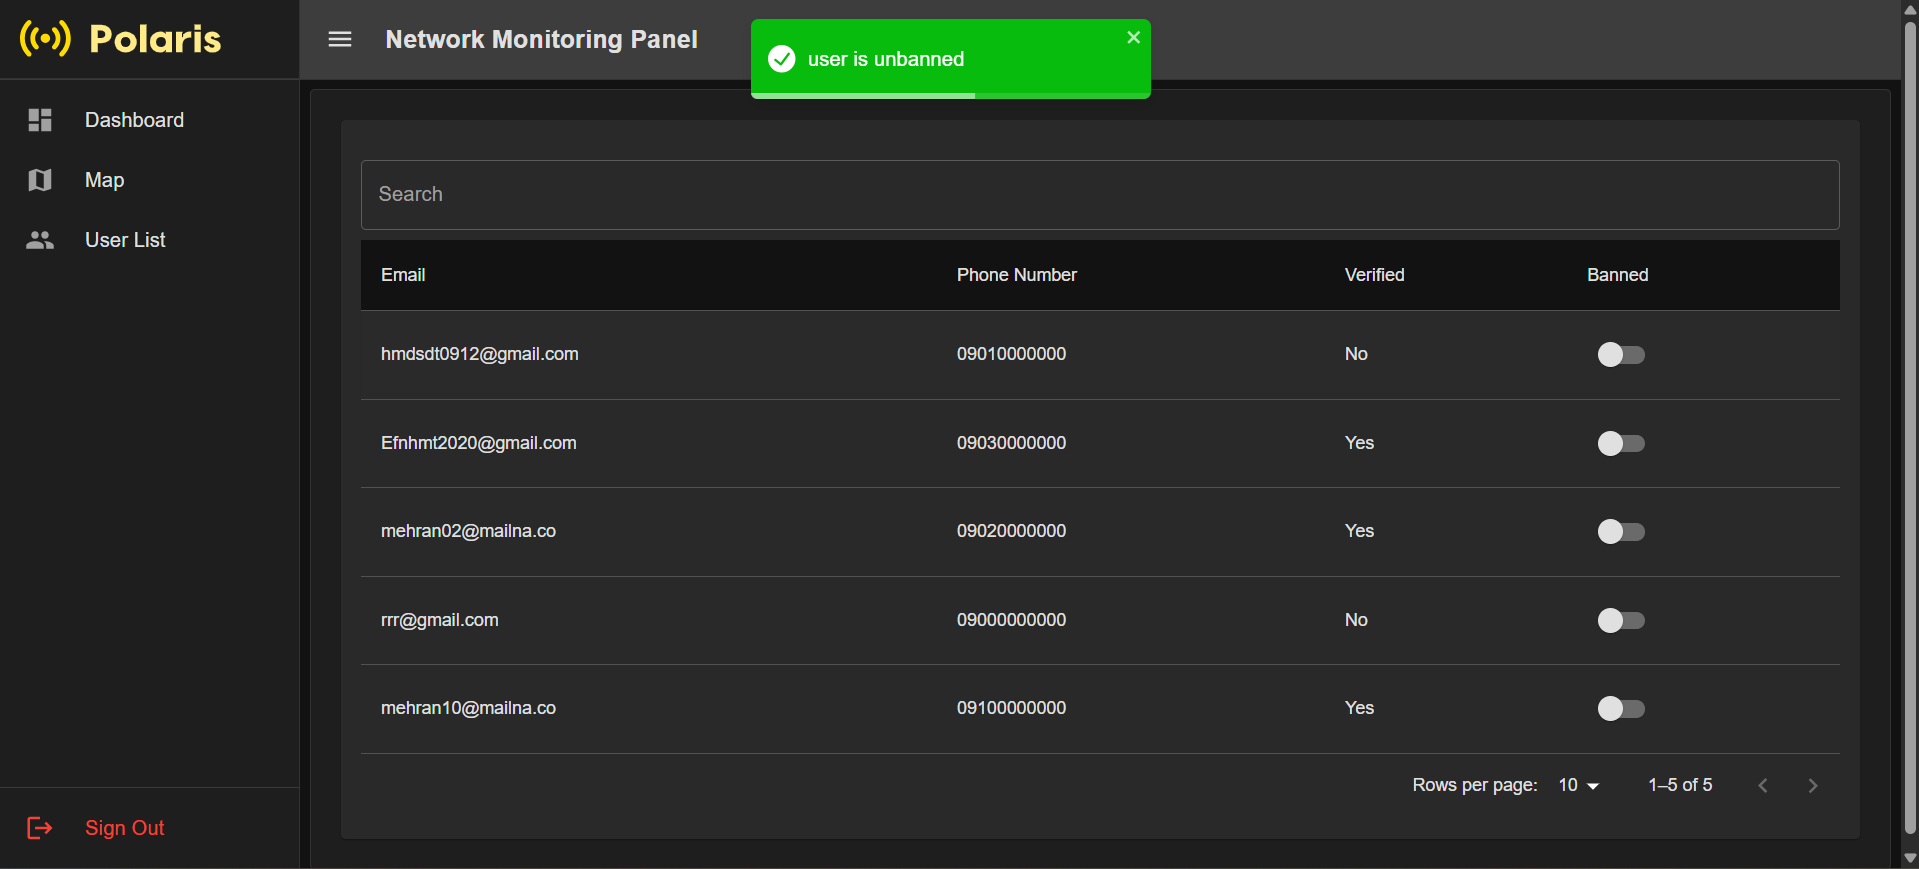
\includegraphics[width=\textwidth]{images/fr-userlist-unban.png}
    		\end{center}
   		همچنین این قابلیت برای مدیر ایجاد شده است که در نوار Search در بین پست الکترونیک کاربران و یا شماره همراه آن‌ها جست و جو کند. برای مثال در تصویر زیر واژه hmd جست و جو شده است و تنها یک نتیجه نمایش داده شده است:
   		\begin{center}
   			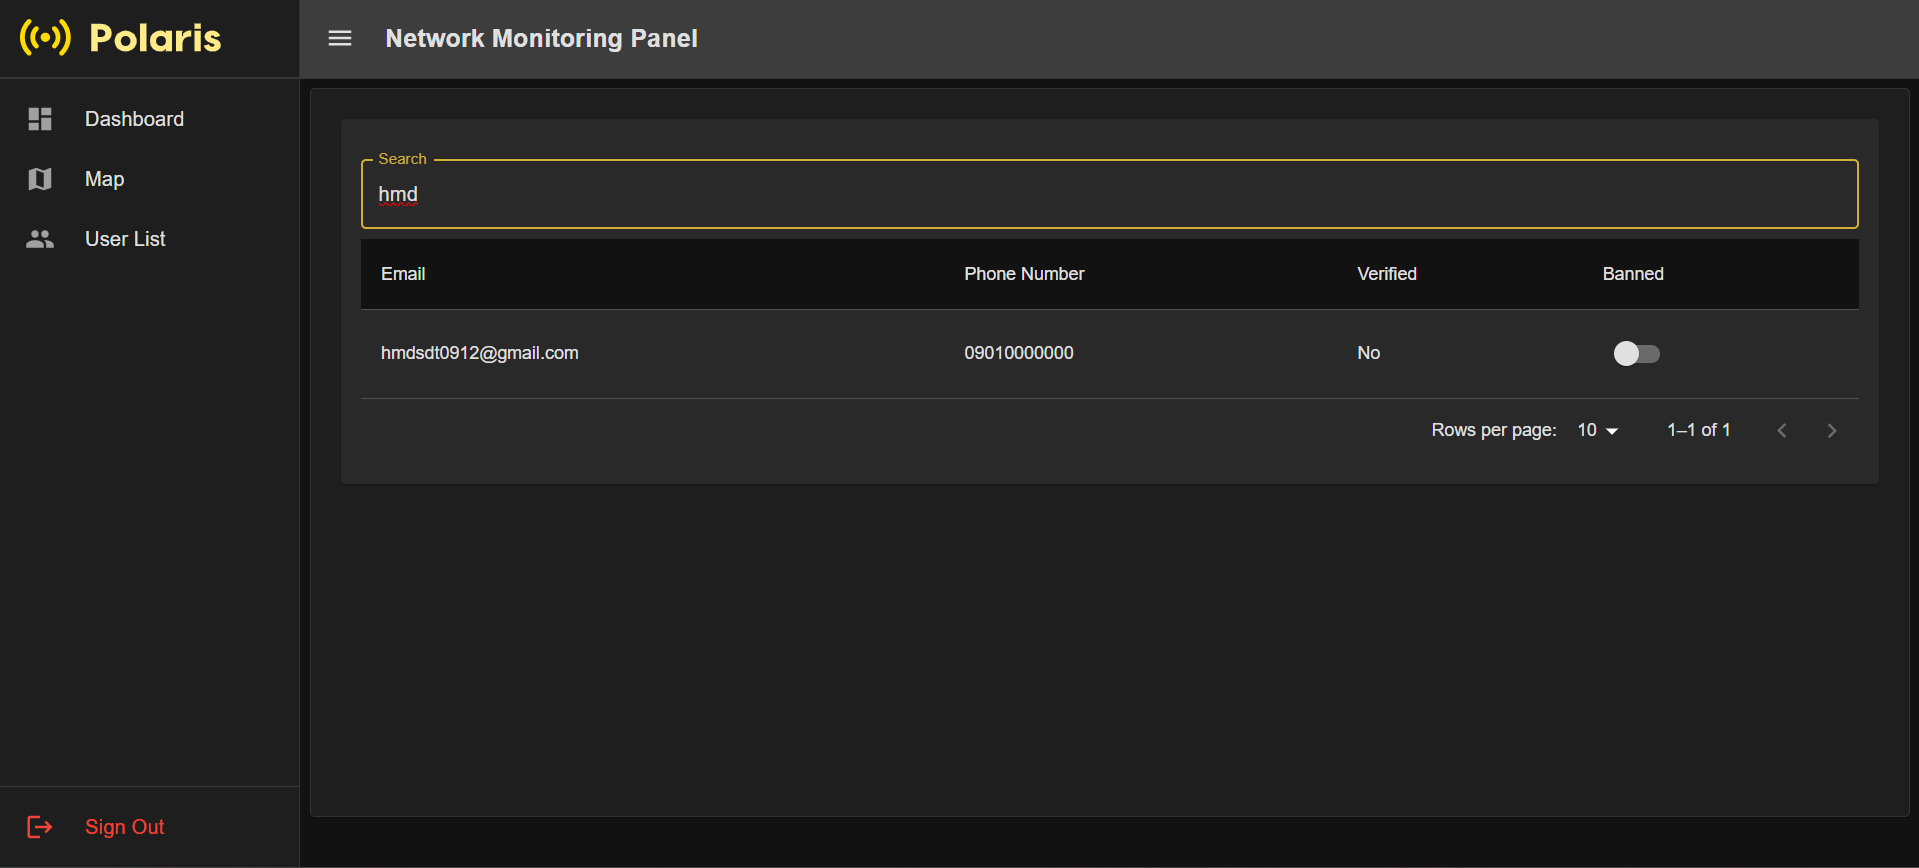
\includegraphics[width=\textwidth]{images/fr-userlist-search.png}
   		\end{center}
   		
    \end{itemize}